%=======================================================================
% paper_v4.tex -- CONTAINER (27 Oct 2026, change of regime). The author writes the text from scratch, to comply with
% the AI policy of JPART. The previous text (paper_v3.tex, secV*.tex, appendix prose, title page), drafted with AI
% assistance, is in _arquivo_texto_IA_2026-10-27/ (README there) and is NOT a source for this text.
% Kept from paper_v3: preamble, title (provisional; see CHECKLIST_VERIFICACAO.md), section files with titles and labels,
% exhibit files (assets/tables), bibliography (references.bib, references_C.bib).
% Working material for the author: referee_EE_2026-10/ESQUELETO.md (facts, numbers, sources; no prose).
% Word limit (JPART): 12,000 words including abstract, tables and references; online appendices excluded. Budget by
% section in ESQUELETO.md, section 0, and in the first lines of each section file (8,350 words of running text).
% Exhibits: tables_V3.tex (body) and tables_V3_appendix.tex (Appendix A) are written by 02_audit/build12_order.py from
% assets/tables/v3w/float_index_v3.csv, in order of first citation; until the text cites them, in the order of the
% index (provisional numbering, renumeracao.md). Tables 3, 6, 7 and Figure 3 of paper_v3 moved to Appendix A.
% Numbers: only those registered in referee_EE_2026-10/NUMEROS_V5.md (with NUMEROS_V3.md and NUMEROS_V4.md).
% Checks after writing: referee_EE_2026-10/CHECKLIST_VERIFICACAO.md.
%=======================================================================

\documentclass[12pt,a4paper]{article}
\input{glyphtounicode}\pdfgentounicode=1

\usepackage[utf8]{inputenc}
\usepackage[T1]{fontenc}
\usepackage{lmodern}
\usepackage[english]{babel}
\usepackage{amsmath,amssymb}
\usepackage{booktabs}
\usepackage{graphicx}
\usepackage{longtable}
\usepackage[margin=1in]{geometry}
\usepackage{setspace}
\usepackage{xurl}
\usepackage[hidelinks]{hyperref}
\usepackage[round]{natbib}
\usepackage{xcolor}
\usepackage[skip=6pt,position=top]{caption}

\graphicspath{{assets/figures/}}

\newcommand{\pending}[1]{\textcolor{red}{[PENDING: #1]}}
\newcommand{\fitbox}[1]{\resizebox{\ifdim\width>\linewidth\linewidth\else\width\fi}{!}{#1}}
\newcommand{\tabnote}[1]{\par\smallskip\noindent\begin{minipage}{\linewidth}\footnotesize\raggedright\textit{Notes:} #1\end{minipage}}

\onehalfspacing

\let\articletitle\title % jrssa-sec1b (06/11/2026), escolha do autor: \title[curto]{} e \keywords{} sao da classe OUP; estas 3 linhas os fazem aceitos pela article e saem na migracao
\renewcommand{\title}[2][]{\articletitle{#2}}
\newcommand{\keywords}[1]{\begin{quotation}\small\noindent\textbf{Keywords:} #1\end{quotation}}
\makeatletter % fecha-jrssa (11/11/2026), pedido do autor: \author[]{}, \address[]{}, \corresp[]{}, \ORCID{}, \orgname{}, \orgaddress{} e \country{} sao da classe OUP; estas linhas os fazem aceitos pela article e saem na migracao
\renewcommand{\author}[2][]{\gdef\@author{#2}}
\newcommand{\address}[2][]{\g@addto@macro\@author{\\[0.5ex]\normalsize #2}}
\newcommand{\corresp}[2][]{\g@addto@macro\@author{\\[0.5ex]\normalsize #2}}
\newcommand{\ORCID}[1]{\\[0.5ex]\normalsize ORCID: \url{https://orcid.org/#1}}
\newcommand{\orgname}[1]{#1}\newcommand{\orgaddress}[1]{#1}\newcommand{\country}[1]{#1}
\makeatother
\title[Measuring compliance with statutory targets]{Measuring Compliance with Statutory Targets: Childcare Access in S\~ao Paulo}

% Identified manuscript: JRSS A reviews single-blind and asks for no separate title page (fecha-jrssa, 11/11/2026).
% Author, affiliation, correspondence and ORCID below, from titlepage_JPART.tex, which is obsolete and kept unchanged.
% Own work is cited in the third person.
\author[1,$\ast$]{Caio Castro\ORCID{0000-0002-6870-0578}}
\address[1]{\orgname{S\~ao Paulo School of Economics -- FGV (FGV--EESP)}, \orgaddress{S\~ao Paulo, \country{Brazil}}}
\corresp[$\ast$]{Corresponding author. \href{mailto:caio.castro@fgv.br}{caio.castro@fgv.br}}
\date{}
\hypersetup{pdfauthor={Caio Castro},pdftitle={Measuring Compliance with Statutory Targets: Childcare Access in S\~ao Paulo},pdfsubject={},pdfkeywords={},pdfcreator={},pdfproducer={}}

\begin{document}

\maketitle

%=======================================================================
\begin{abstract}
A numerical target written into law looks verifiable, but whether it is met depends on conventions the law does not fix. One is the date on which a waiting list is counted, and it moves the result. We study Goal~5 of S\~ao Paulo's 2015 Municipal Education Plan, which sets two childcare requirements and applies whichever is greater. Combining the published waiting-list series, enrolment records and alternative population estimates, we compute the verdict under alternative conventions. Across our measurement grid, Goal~5 compliance is specification-dependent in 2019--2022, whereas no specification in that grid indicates compliance in any evaluable year in 2010--2018; before September 2019, only the published waiting-list series is available. Between 2014 and 2017, the published list fell by 53.2\% when counted in December and by 17.5\% to 20.5\% in other quarters. The municipality's 2023 review declared the goal achieved, stated that it had been met since 2015, and published no formula; no specification reproduces that verdict. A verifiable indicator must define eligible requests and service, and fix the time allowed, observation date, enrolment universe, population source and vintage, and the rule combining both requirements.
\end{abstract}
\keywords{administrative data; childcare; official statistics; performance measurement; policy targets; waiting lists}

\clearpage

\section{Introduction}\label{sec:intro}

A numerical target written into law looks verifiable. It names a number, a population and a deadline, and it seems to ask only that someone compute the corresponding statistic and compare it with the threshold. In effect, such a target is a legal requirement to produce an official statistic, written before that statistic has been defined. What counts as a member of the population, as a request, as service and as the moment of observation depends on conventions that the law usually leaves open. Someone has to settle them after the law is passed, and that someone may be the agency whose performance the target is meant to assess. Until they are settled, the question of whether the target has been met has no unique answer, and a law that appeared verifiable is not.

The date of observation is the clearest example. When a target is set on the stock of a waiting list, the stock has to be counted on a particular day, and the answer moves with the day. Statistical systems that publish waiting lists usually fix that day by rule. Social housing registers kept by English local authorities are reported as of 31 March, Norwegian kindergarten waiting lists as of 15 December, and waiting times in the English National Health Service at the end of each reporting period \citep{mhclg_table600,ssb13632,nhs_rtt_mar26}. A fixed date makes counts comparable from one year to the next; it does not make any particular date neutral. The childcare waiting list analysed in this paper shows how much the choice can matter. Between 2014 and 2017, the stock counted on a single day fell by 53.2\% when that day was in December and by between 17.5\% and 20.5\% when it was in any other quarter, so that the percentage decline measured in December is 3.03 times that measured in September. Measures of flow, dated by the request rather than by the count, are much less sensitive to the ending month: for them, the ratio of the December change to the September change lies between 0.75 and 1.11. A law that sets a target on a stock without fixing the date leaves the verdict to whoever chooses the day. That is a matter of indicator design, and it arises whatever the service and whatever the country.

Much of this is familiar in outline. \citet{chun2005goal} describe evaluative goal ambiguity, the interpretive leeway that the goals of public agencies allow when progress towards them is judged. \citet{bevan2006measured} show that a regime of targets rests on the assumption that what is measured is what matters, and document the gaming that followed in the English health service. \citet{bird2005performance} set out what a performance monitoring protocol must specify for an indicator to be interpretable, from its definition to the reporting of its uncertainty. Work on multiverse and specification curve analysis recommends reporting results across the set of defensible analytic choices rather than for a single preferred one \citep{steegen2016increasing,simonsohn2020specification}. Together, these studies establish that public goals can be ambiguous, that indicators respond to the uses made of them and that conclusions can depend on choices taken before any number is reported. They seldom have the administrative microdata needed to enumerate the conventions behind a particular statutory target and to compute the verdict under each of them. In specification analysis, moreover, the alternatives usually concern estimation; here they arise earlier, when a legal objective is turned into a population, an event and a date. What microdata add is an arithmetic demonstration, in a case where the law, the data and an official verdict can all be examined, that the legal verdict depends on the convention.

Our case is S\~ao Paulo, where three conditions that rarely occur together are met. First, the ambiguity is in the statutory text. Goal~5 of the city's 2015 Municipal Education Plan requires childcare for at least 75\% of children aged 0 to 3 years and 11 months or for 100\% of registered demand, whichever is greater \citep{saopaulo2015pme}. The first requirement counts children whether or not their families have applied, the second rests on requests the administration can observe, and the clause that joins them admits more than one reading. Second, the inputs exist at the level of detail the conventions require. The municipality publishes its waiting list on regular dates and keeps centralized individual records of requests and of enrolments, and the School Census distinguishes enrolment by school network, so each convention can be computed rather than only argued about. Third, there is an official verdict to check: in 2023, the municipality's review of the plan declared Goal~5 achieved \citep{saopaulo2023conferencia}.

We make explicit the six conventions that the law leaves open: which waiting list counts as registered demand, the date on which it is observed, the source of enrolment for the demand requirement, the school networks counted for population coverage, the population series used as the denominator, and the rule that combines the two requirements. The inputs are the published waiting-list series, the municipality's enrolment publications, the School Census, live birth registrations, and demographic censuses and projections. The main grid fixes the December reference date, enrolment across all networks for the population requirement and the reading under which only the larger requirement binds, and crosses the remaining choices into 12 combinations. An extended grid in the appendix adds alternative dates, enrolment universes and readings of the clause, for 144 combinations. For each combination, we compute the verdict in every year in which its inputs exist. Each combination is a convention an agency could adopt with the data available. The grid shows how far the verdict depends on those conventions; it is not a distribution of legally valid readings, and we do not weight its cells.

Across our measurement grid, Goal~5 compliance is specification-dependent in 2019--2022, whereas no specification in that grid indicates compliance in any evaluable year in 2010--2018; before September 2019, only the published waiting-list series is available. Of the 12 main combinations, seven indicate compliance in at least one evaluable year and five never do, and none of the 648 evaluable combination-year observations for 2010--2018 in the extended grid indicates compliance. These statements hold within the documented grid. A mechanically rescaled population projection, which we exclude under an explicit provenance criterion, would indicate compliance in 2018. The 2023 review declared the goal achieved and reported that its threshold had been reached since 2015, without publishing its formula. No specification in the grid reproduces that account. The ratio of December municipal enrolment to the sum of that enrolment and the published waiting list reproduces six of the eight values the review reports, but a 75\% threshold on that ratio is not the statutory obligation to serve all registered demand, and it does not identify which requirement binds. Applied to the same ratio, the reference date alone moves the first year above 75\% from 2015 with December counts to 2018 with September counts.

What follows from these results is a list of what a verifiable indicator has to fix: the definitions of an eligible request and of service, the time within which a request must be met, the date of observation, the enrolment universe, the source and vintage of the population data, and the rule that combines the two requirements. Nothing on that list is specific to S\~ao Paulo or to childcare, since it applies to any target set on a waiting list or on the coverage of an eligible population. Brazil's new National Education Plan, enacted in April 2026, requires childcare to meet 100\% of expressed demand without defining the term, and the indicators that will measure it are still being specified \citep{brasil2026pne,mec2026portaria701}.

Section~\ref{sec:institutions} describes the legal and institutional setting, Section~\ref{sec:data} the data and Section~\ref{sec:goal} the verdict across the grid. Sections~\ref{sec:series} to~\ref{sec:service} examine the published stock, the coverage of the request record and the timing of requests and referrals, Section~\ref{sec:scope} sets out the limits of the evidence, Section~\ref{sec:indicators} turns the findings into indicators and a publication protocol, and Section~\ref{sec:conclusion} concludes.

% secV2_setting.tex -- Section 2. CONTAINER (27 Oct 2026): text to be written by the author.
% Word budget: 800 words (JPART count: running text, footnotes and citations as printed).
% Outline, numbers and sources: referee_EE_2026-10/ESQUELETO.md, section 2. The archived text
% (_arquivo_texto_IA_2026-10-27/) is not a source.

\section{Institutional and legal setting}\label{sec:institutions}

Childcare for children below age four is not compulsory in Brazil, unlike preschool for four- and five-year-olds, which became compulsory under the 2009 constitutional amendment \citep{brasil2009ec59}. Access to early-childhood education is nevertheless an enforceable right. In 2022, Brazil's Supreme Federal Court held that public childcare and preschool provision can be demanded individually (Theme 548, RE 1,008,166) \citep{stf2022tema548}. Registration consequently captures families' expressed requests for a public place, not the population of all children who might benefit from childcare. The 2014 National Education Plan established a population target of serving at least 50\% of children under four \citep{brasil2014pne}.

S\~ao Paulo's municipal system uses three arrangements: directly operated centres (\emph{rede direta}), municipally owned centres under private management (\emph{rede indireta}), and private centres operating under municipal agreements (\emph{rede conveniada}). Childcare places are divided among Ber\c{c}\'ario I, Ber\c{c}\'ario II, Minigrupo I, and Minigrupo II according to age at the March 31 cut-off. The corresponding adult-to-child ratios are 1:7 for ages 0--11 months, 1:9 for 12--23 months, 1:12 for 24--35 months, and 1:25 for 36--47 months \citep{sme2020in36}. Between 88\% and 89\% of Ber\c{c}\'ario I classes operate exactly at their authorized class size, compared with 23\% to 25\% of Minigrupo II classes (Table~\ref{tab:T6a_modulo}), while the ratio of enrolment to authorized places ranges from 0.93 to 0.996 (Table~\ref{tab:T6b_ratio}). Because assignments must also match a child's age group, vacancies are not necessarily interchangeable across children.

Families can apply throughout the year at no charge. The registration system uses the child's address to identify geographically eligible centres rather than collecting a ranked list of preferred centres. At each centre, applications are ordered chronologically within priority categories, including judicial orders and specified vulnerability or special-needs criteria. Families may also elect to remain registered for a particular centre after being offered a place elsewhere, preserving the original protocol order for that centre under a 2011 municipal ordinance \citep{sme2011portaria3478}. A centre-specific request may therefore remain on the published list despite an alternative offer. Geographical assignment rules have changed over time; we do not impose a fixed distance radius across the sample.

Referrals can occur throughout the year, but the allocation calendar is highly seasonal. Of first referrals dated 2013--2017, 50.5\% occurred in December (Table~\ref{tab:calendar}) and another 15.8\% in January--February, whereas only 5.0\% of first applications occurred in December. We refer to December--February as the main allocation round. A year-end list count therefore reflects the timing of referrals as well as the stock of unresolved applications. Childcare provision also expanded substantially: all-network childcare-stage enrolment increased from 170,720 in 2010 to 365,854 in 2018, across a change in the treatment of Minigrupo II in 2011. Authorized places for children under four rose by 58\% from the first semester of 2013 to the first semester of 2019 (Tables~\ref{tab:T2a_capacidade} and~\ref{tab:R_capcheck}; Figure~\ref{fig:F7}). Meanwhile, annual live births declined by 6.3\% between their 2011 peak and 2018. Between 2013 and 2019, the number of partner-operated and indirectly managed centres increased from 1,223 to 2,004, while directly managed centres declined from 418 to 402 (Table~\ref{tab:T7a_ceis}), and places per eligible child rose from 0.307 to 0.514, with a descriptive decomposition assigning 86\% of this increase to capacity growth and 14\% to the decline in the eligible population (Table~\ref{tab:S6c_cobertura}). The distribution of enrolment recorded in the municipal childcare request data also shifted towards private centres operating under municipal agreements, while the shares of directly managed and indirectly managed municipal centres declined (Table~\ref{tab:T5c_modal}). These trends jointly affect observed enrolment rates and queue counts but do not, by themselves, identify policy effects.

S\~ao Paulo adopted its Municipal Education Plan (PME) under Law 16,271 of September 17, 2015, establishing 13 goals over a ten-year horizon. Goal~5 mandates universal preschool for four- and five-year-olds by 2016 and, during the plan's validity, childcare provision for at least 75\% of children aged 0--3 years and 11 months or 100\% of registered demand, whichever is greater \citep{saopaulo2015pme}. The childcare target exceeds the national plan's population threshold; Law 17,437/2020 later extended the PME goal deadlines by two years \citep{saopaulo2020lei17437}. Strategy 5.1 calls for expansion through direct, indirect, and partnered centres.

The law specifies neither the definition of registered demand, nor a population denominator, nor a rule for reconciling enrolment measures. Subsequent documents introduced monitoring conventions. Ordinance 7,972 of the Municipal Education Secretariat (SME), issued in December 2016, organizes annual monitoring in January--February, with a July round for indicators relying on the School Census, and instructs that indicators be recorded as of December 31 \citep{sme2016portaria7972}. The 2016 baseline report uses December 31, 2015 as its reference date, without a published formula permitting independent reconstruction of Goal~5's compliance measure \citep{sme2016linhabase}. The municipality's 2023 conference review classified Goal~5 as achieved \citep{saopaulo2023conferencia}. Section~\ref{sec:goal} examines the measurement conventions necessary to interpret that classification.

% secV3_data.tex -- Section 3. CONTAINER (27 Oct 2026): text to be written by the author.
% Word budget: 550 words (JPART count: running text, footnotes and citations as printed).
% Outline, numbers and sources: referee_EE_2026-10/ESQUELETO.md, section 3. The archived text
% (_arquivo_texto_IA_2026-10-27/) is not a source.

\section{Data}\label{sec:data}

We combine child-level administrative records provided by the SME with aggregate administrative publications, school enrolment data, and demographic records. We distinguish the \emph{request record}, which tracks individual requests, from the \emph{published waiting list}, which reports administrative counts at specific dates. Neither measures all families potentially interested in childcare.

The application files for 2010--2018 contain 3,298,064 records, including child identifiers, application dates, location, and dated referral and enrolment events observed through November 2019. We retain the first valid application per child, yielding 1,524,560 children (Table~\ref{tab:T1_fila}). Our unit of analysis for application flows is thus the child's first \emph{request}, not each administrative record. Because coverage is incomplete in the earliest years, analyses of entries and subsequent trajectories focus on first requests made from July 2012 onward. A \emph{referral} is an offer or assignment of a place, distinct from an effective \emph{enrolment}; children may also exit the childcare list upon reaching 47 months. Application timestamps are recorded to the second, although 2.7\% of first requests share a recorded second with another request (Table~\ref{tab:N1}). A guardian's CPF is recorded for 98.1\% of these children; we treat the identifier as present when it is non-missing and positive, without verifying its check digit. Separately provided Escola On-Line (EOL) enrolment records, linked by child identifier, permit comparisons with enrolment information recorded outside the application extract. Neither child-level source is publicly available. A separate capacity panel covers 2,734 centres across 13 semesters, with 86,982 centre--semester--age-group observations on authorized places.

We reconstruct the published series from the SME's original open-data files for 2006--2016 and subsequent administrative spreadsheets \citep{sme_dados_abertos,sme_demanda_escolar}. Municipal Law 14,127/2006 and Decree 47,155/2006 mandate quarterly publication of demand statistics by district and educational stage \citep{saopaulo2006lei14127}. SME Technical Note 01/2017 \citep{sme2017nt01} defines \emph{demanda} as registered applications without a referral, excluding cases with a referral, withdrawal or refusal, expired requests, school-transfer applications, and residents of other municipalities. The published figures are snapshots of the administrative system, rather than measures of unexpressed demand. Our assembled series contains 89 snapshots, quarterly through 2022 and bimonthly from 2023. Table~\ref{tab:series} reports the quarterly counts through 2022 and the June and December counts from 2023. Among 43 corresponding PDF releases checked against open-data totals, 37 match; the remaining six have formats or disaggregations that preclude a direct comparison. We use the underlying administrative tabulations.

For population coverage, the May School Census provides childcare-stage enrolment across all school networks and a municipal-and-partnered subset \citep{inep_censo_escolar_c}. For registered-demand calculations, we compare the SME's December enrolment series with the municipal-and-partnered School Census count; their reference dates and coverage differ. Population inputs comprise district-level live births from SINASC, the 2010 and 2022 Demographic Censuses, and SEADE's published age-specific projections \citep{sms_sinasc_tabnet,ibge_sidra1378,ibge_sidra9514,seade_idade_escolar}. Our principal under-four population series scales birth cohorts to both Census benchmarks. Alternatives interpolate directly between the two Census counts or between SEADE projections published for 2005, 2010, 2015, 2020, and 2025. Section~\ref{sec:goal} defines these constructions and the resulting compliance measures.

The application records were also used in \citet{soares2021ecd}, which studies childcare expansion and child outcomes. Our research question is different: we do not identify the effect of a programme, but examine whether a statutory performance claim is reproducible.

% secV7_goal.tex -- Section 4. CONTAINER (27 Oct 2026): text to be written by the author.
% Word budget: 2,000 words (JPART count: running text, footnotes and citations as printed).
% Outline, numbers and sources: referee_EE_2026-10/ESQUELETO.md, section 4. The archived text
% (_arquivo_texto_IA_2026-10-27/) is not a source.
% \label{sec:pandemic} is defined in this section, on the subsection on the post-2019 period and the
% official review; the note of Table A13 (V3w_indet_full) refers to it.

\section{What Goal~5 leaves open}\label{sec:goal}

Goal~5 of S\~ao Paulo's Municipal Education Plan requires the provision of childcare to at least 75\% of children aged 0--3 years and 11 months or to 100\% of registered demand, whichever is greater \citep{saopaulo2015pme}. The law leaves the operational conventions needed to assess compliance unspecified. Across our measurement grid, Goal~5 compliance is specification-dependent in 2019--2022, whereas no specification in that grid indicates compliance in any evaluable year in 2010--2018; before September 2019, only the published waiting-list series is available.

\subsection{Operationalizing the two requirements}

Let $P_t$ denote the estimated number of children below age four in year $t$, $E^A_t$ the number enrolled under the coverage definition used for the population requirement, $E^B_t$ the number enrolled under the administrative definition used for registered demand, and $L_t$ the number of children remaining on the relevant waiting list. The two requirements imply quantities $T^A_t=0.75P_t$ and $T^B_t=E^B_t+L_t$. A natural implementation compares $T^A_t$ and $T^B_t$, assesses $E^A_t\geq 0.75P_t$ when the first is larger, and requires $L_t=0$ when the second is larger. The latter condition is equivalent, for positive enrolment, to $E^B_t/(E^B_t+L_t)=1$. This rule is an analytical reconstruction, not a statutory formula. Because $E^A_t$ and $E^B_t$ may differ in universe or date, their comparison requires another convention absent from the law.

The waiting list presents the first ambiguity. The published series includes centre-specific requests even when families are offered places elsewhere; a narrower series, available only from September 2019, excludes them. These families therefore count as having unmet demand only in the published series. Across 89 published snapshots, the full list is never zero. By contrast, the narrower list is zero in each December observation from 2020 through 2025, while remaining positive in the other 30 observations between September 2019 and August 2026. Whether the queue is empty thus depends on its definition, and the series cover different periods.

Goal~5 does not specify a reference date. A subsequent municipal monitoring ordinance records indicators as of December 31 \citep{sme2016portaria7972}, and the plan's baseline report uses December 31, 2015 \citep{sme2016linhabase}; December is consequently our principal specification. In 2019, the published waiting-list count fell from 75,267 in September to 9,670 in December. We examine September snapshots and annual averages in the appendix.

The enrolment quantities require distinct choices. For the population requirement, the School Census permits a count of children enrolled in the childcare stage across all school networks, or a narrower count covering municipal and publicly partnered providers. Article~7 of the municipal law states that the plan's goals apply to all educational systems in the municipality. We read this as supporting the all-network interpretation for the main analysis, while recognizing that ``systems'' and ``networks'' are not defined as equivalent in the statute; the municipal-and-partnered interpretation remains a sensitivity check. The choice matters: using our principal population series, all-network childcare-stage enrolment reaches 76.8\% of children under four in 2021, whereas the municipal-and-partnered measure reaches only 70.3\%. A classification break prevents a comparable municipal-and-partnered series after 2021. An alternative age-based count, including enrolment at any stage, yields 78.6\% in 2022, against 83.8\% for the childcare-stage measure (Table~\ref{tab:arms}).

For the registered-demand requirement, enrolment may come from the municipal secretariat's December publication, which also reports the waiting list, or from municipal-and-partnered enrolment in the May School Census. The sources differ in date and coverage. In 2021 the secretariat reported 385,100 municipal childcare enrolments in December, exceeding even the 377,862 enrolments across all networks reported by the May School Census. This need not indicate error in either source. Finally, ``whichever is greater'' can mean testing only the larger requirement, as in our main specification, or requiring an empty list regardless. We retain both readings.

\subsection{The denominator is not specified by the law}

The population denominator is a sixth, independent choice. Article~4 of the municipal law refers to the most recent \emph{basic and higher education censuses available on the date of the law's publication} (September 17, 2015); it does not select a demographic census, a population projection, or a procedure for estimating children under four. Our principal series combines civil registration of live births with the 2010 and 2022 Demographic Censuses. For a School Census observation in May of year $t$, we count births from June of $t-4$ through May of $t$ and divide this four-year pool by a scaling factor. The factor is the ratio of the corresponding birth pool to the census population aged 0--3 at the two benchmark years (1.228 in 2010 and 1.278 in 2022), interpolated linearly between them. By construction the resulting series reproduces the two demographic census benchmarks. It preserves cohort variation while assuming a linear scaling factor.

We compare this measure with two alternatives (Table~\ref{tab:armArob}). The first interpolates the 0--3 population directly between the two Demographic Censuses, from 564,210 in 2010 to 464,826 in 2022, without using the intervening birth series. The second interpolates published SEADE projections. Our grid admits two series types: reconstructions calibrated to both Demographic Census benchmarks, and interpolations of independently published population projections. This provenance criterion does not select series by their proximity to a single benchmark. The SEADE interpolation is included because the secretariat cites SEADE estimates when describing coverage, although Goal~5 neither requires nor excludes them. Our interpolation of SEADE's published projections yields 531,819 children in 2022, 14.4\% above the 2022 Demographic Census count of 464,826; this is a discrepancy, not an estimate of SEADE's error. A SEADE series mechanically rescaled to match only the 2022 Census satisfies neither criterion: it gives 498,176 children in 2010, 11.7\% below the Census count of 564,210. We exclude it from the grid, but note that it yields compliance in 2018 under two December published-list specifications. This exclusion is not mandated by law.

These denominators matter near the threshold. With the births-scaled series, all-network childcare-stage enrolment rises from 67.4\% in 2018 to 73.0\% in 2019, 74.1\% in 2020, 76.8\% in 2021, and 83.8\% in 2022 (Table~\ref{tab:arms}). A population 2.6\% lower in 2019 or 1.2\% lower in 2020 would move the first requirement to 75\%; conversely, a population 2.4\% higher in 2021 would move it back to the threshold. For perspective, the post-enumeration evaluation of Brazil's 2022 Census reports a national net coverage error of 8.3\%, with estimates around 10\% for children aged up to four \citep{agenciabrasil2024ppe}. These national rates cannot be applied as corrections for S\~ao Paulo, but underscore why near-threshold classifications are sensitive to measurement.

\subsection{Compliance across specifications}

Table~\ref{tab:indet} evaluates 12 combinations holding constant the December reference count, whatever its printed extraction date, all-network enrolment for the population requirement, and the rule that only the larger of the two requirements binds. The combinations vary the published versus narrower list, the three population series, and the secretariat versus School Census enrolment measure for registered demand. Seven combinations meet the goal in at least one observable year; five meet it in none. The earliest qualifying year is 2019 in four combinations and 2021 in three. None classifies a year before 2019 as compliant within the observations that can be evaluated.

The classifications differ across these combinations. With the published list, births-scaled population, and secretariat enrolment, the goal is not met in any evaluable year; replacing secretariat enrolment with the School Census changes the classification for 2021. Using the linearly interpolated population instead gives compliance in 2019 alone with secretariat enrolment and in 2019--2021 with School Census enrolment. Under the narrower list and births-scaled population, secretariat enrolment yields compliance in 2021--2022, whereas the School Census yields 2021 only. Combining the narrower list with the linear population series gives compliance in 2019--2022 under secretariat enrolment and in 2019--2021 under School Census enrolment. None of the four combinations using the SEADE projection meets the goal. The published-list, linear-population, secretariat-enrolment specification qualifies in 2019 but not later, yielding a nonmonotonic classification.

{\emergencystretch=1em Table~\ref{tab:indetfull} extends this exercise to September observations, annual-average lists, municipal-and-partnered enrolment for the population requirement, and the interpretation that registered demand must always be fully served. The resulting grid contains 144 combinations. The grid enumerates specifications; it is neither a distribution of legally valid interpretations nor a statistical confidence interval \citep{steegen2016increasing,simonsohn2020specification}. Of the 144 combinations, 21 meet the goal in at least one evaluable year and 123 never do; four exhibit a transition from compliance to noncompliance in a later evaluable year. Among combinations that ever qualify, four first do so in 2019, eight in 2020, and nine in 2021. None first qualifies in 2022. In the 2010--2018 period, 72 combinations can be evaluated, all necessarily based on the published list because the narrower series did not yet exist. None of the resulting 648 combination-year observations meets the goal. Evaluable years differ: the narrower list starts in 2019 and the relevant School Census split ends in 2021. A ``never'' entry means never among observed, evaluable years, not a verified failure at all dates.\par}

\subsection{The post-2019 period and the official review}\label{sec:pandemic}

All positive compliance classifications in our specification grid occur in 2019--2022, a period combining enrolment changes, declining birth cohorts, and the disruption of the COVID-19 pandemic. The published September waiting list falls from 75,267 in 2019 to 6,670 in 2020, while secretariat enrolment increases by 20,490. Enrolment plus the published waiting-list count consequently falls by 11.7\%, compared with a 2.8\% decline in the relevant birth pool. The December list falls from 9,670 in 2019 to 540 in 2020; over the same interval, December municipal enrolment increases by 29,179. Births in 2020, 2021, and 2022 are, respectively, 7.2\%, 13.8\%, and 16.7\% below their 2019 level. These movements do not identify changes in preferences, applications, capacity, or pandemic effects.

Without post-2018 individual applications, we cannot distinguish fewer registrations from greater outflows or recording changes. Stock accounting provides a lower bound on first-half entries: increases from December to June imply at least 29,213 entries in 2019, 13,062 in 2020, 8,227 in 2021, and 4,166 in 2022, even before allowing for exits during the interval. Where individual records exist, this bound captures only 24--42\% of first requests. It establishes continuing inflows but identifies neither pandemic effects nor counterfactual compliance. Furthermore, 14 of the 21 specifications that ever qualify do so only in 2020--2021, but none of those 14 can be evaluated in 2022. Their observed patterns cannot be interpreted as evidence of a subsequent reversal.

The municipality's 2023 review nonetheless classified Goal~5 as achieved and reported that the 75\% threshold had been reached as early as 2015 \citep{saopaulo2023conferencia}. Its published indicator was labelled the share of registered childcare demand served, with December as the reference month, rather than an explicit test of the legal maximum of the two requirements. The review did not publish the indicator's formula. We find that $E^B_t/(E^B_t+L_t)$, constructed from December municipal enrolments and the published list, reproduces six of its eight reported values for 2015--2022 to two decimal places. The exceptions are 2019 (96.31\% reported versus 97.28\% reconstructed) and 2022 (99.99\% versus approximately 99.81\%). Published documentation does not explain the discrepancies. Crucially, this indicator neither identifies the binding statutory requirement nor tests compliance with it. The review's classification thus cannot be recovered as compliance with any of the 144 specifications examined here, even though much of its reported series is numerically close to a recognizable administrative ratio.

The availability of these retrospective specifications to the 2023 reviewers is unknown: the publication date of the age-specific 2022 Census data has not been verified. None is a legally definitive indicator. Rather, the same statutory wording supports materially different empirical classifications, and the administrative review does not document the additional conventions necessary to adjudicate among them. A reproducible judgement about Goal~5 therefore requires making these six conventions explicit.

% secV6_series.tex -- Section 5. CONTAINER (27 Oct 2026): text to be written by the author.
% Word budget: 700 words (JPART count: running text, footnotes and citations as printed).
% Outline, numbers and sources: referee_EE_2026-10/ESQUELETO.md, section 5. The archived text
% (_arquivo_texto_IA_2026-10-27/) is not a source.

\section{The published number}\label{sec:series}\label{sec:stock}

The published waiting list is an administrative count whose definition and observation date have changed over time. In 2011, the inclusion of Minigrupo II altered the population covered by childcare statistics \citep{sme2011nota_reorg}. A July ordinance allowed families already referred elsewhere to retain a centre-specific request \citep{sme2011portaria3478}; an October publication identified these cases as \emph{demanda preferencial} \citep{sme2011nota_pref}. In March 2012, SME distinguished the stock of requests carried over from the previous year from new registrations and identified cases pending documentation \citep{sme2012nota}. From September 2019, releases separated requests with and without a specific-centre preference; from September 2020, they also distinguished waiting times up to and above 30 days. Publication changed from quarterly to bimonthly in 2023. Accordingly, levels cannot be treated as a consistently defined time series across 2011 or 2019 (Table~\ref{tab:series}). The distinction remains consequential: a December 2020 municipal announcement described the narrower waiting list as cleared while acknowledging 540 children waiting for a specific centre \citep{saopaulo2020fila}. The published list itself was not zero. The 2025--2028 municipal goals programme uses a still narrower measure: requests without a specific-centre preference pending for more than 30 days \citep{sme_metas2025}.

Even within periods of comparable definitions, the date of observation substantially changes the count. December has the year's lowest published waiting-list count in 17 of the 19 years from 2007 to 2025. Between 2013 and 2017, the December count fell from 96,696 to 44,092, a 54.4\% reduction; the corresponding changes in March, June, and September were only 14.9\%, 18.1\%, and 15.7\% (Table~\ref{tab:series}). The within-year decline from September to December rose from 38.4\% in 2013 to 87.2\% in 2019. The annual mean of the four quarterly counts declined by 23.9\% between 2013 and 2017, from 121,087 to 92,158 (Table~\ref{tab:series}). Thus, both the measured level and its apparent trend depend on the month chosen.

Individual administrative records allow us to investigate the mechanism for 2013--2018. We reconstruct the stock of unresolved first requests at each quarter-end using dated entries and exits from the request record. Across those quarters, reconstructed counts are 87--96\% of the corresponding published counts (Table~\ref{tab:recon}). They exhibit the same seasonal pattern: from 2013 to 2017, the reconstructed December stock fell by 53\%, against declines of 16--19\% in the other quarters; Table~\ref{tab:decomp} reports the December and September levels. The December decline is therefore not confined to the publication series, although the differences in levels remain unexplained.

A stock--flow decomposition identifies referrals as the principal source of the year-end reduction. Over 2013--2018, 97.4\% of recorded exits between September and December are referrals, compared with 2.3\% attributable to ageing out and 0.3\% to recorded withdrawals (Table~\ref{tab:decomp}). For 2013--2017, referrals during this interval average 94,262 per year, equivalent to 71.2\% of the reconstructed September stock; approximately 32,150 new requests also enter during the interval. These movements are consistent with the main allocation round described in Section~\ref{sec:institutions}, rather than a year-end purge of registrations. The decomposition is unavailable after 2018 and does not establish the mechanism in later years.

The publication's extraction date further affects what a ``December'' observation captures. For 2014--2018, at least 99.2\% of referrals occurring in December had already taken place by the corresponding extraction date (Table~\ref{tab:decomp}). These snapshots therefore follow the December wave of referrals, though they precede the subsequent January--February wave. The extraction convention is not uniform: of 18 December editions with a printed date, ten use December 31, while other dates range from November 30 to December 28 (Table~\ref{tab:dates}). These dates establish variation, not its administrative cause.

The choice carries directly into assessments of Goal~5. Applying the 75\% threshold used in the municipality's 2023 review to the share $E^B_t/(E^B_t+L_t)$ yields a first crossing in 2015 with December counts, in 2018 with September counts, and in 2017 using the annual mean of published counts (Table~\ref{tab:series}). This threshold is not the law's requirement to serve 100\% of registered demand. The December count, taken after the year's principal referral wave, consequently makes the review's criterion appear to be reached earlier (Figure~\ref{fig:goal}). It is an observable mechanism behind the reference-date sensitivity documented in Section~\ref{sec:goal}, not evidence that the statutory goal was met.

% secV4_coverage.tex -- Section 6. CONTAINER (27 Oct 2026): text to be written by the author.
% Word budget: 400 words (JPART count: running text, footnotes and citations as printed).
% Outline, numbers and sources: referee_EE_2026-10/ESQUELETO.md, section 6. The archived text
% (_arquivo_texto_IA_2026-10-27/) is not a source.

\section{Coverage of the request record}\label{sec:coverage}

The request record underpins the cohort trends analysed below and the proposed measure of application flows, but not the Goal~5 compliance exercise: every specification in our measurement grid relies on published aggregate waiting-list counts rather than individual application records. The supplied files are not SME's live system. Stocks reconstructed from them for 2010 reach only 20--33\% of the published list (Table~\ref{tab:recon}), which indicates incomplete coverage in the supplied records, though not necessarily in the underlying administrative system.

We assess coverage independently by matching first requests to childcare entrants in Escola On-Line (EOL) enrolment records. The matched share is 42.1\%, 47.9\%, and 57.2\% in 2010, 2011, and 2012, respectively, against 98.6--99.9\% in 2013--2018 (Table~\ref{tab:coverage}; Figure~\ref{fig:coverage}). The discontinuity is concentrated in February: only 41.4\% of 87,228 February 2012 entrants have a matching request, versus 98.3\% of 33,773 entrants in other months. Across centre types, February coverage rises from 32.0--43.6\% in 2012 to 95.8--98.8\% in 2013 (Table~\ref{tab:covtype}), and, among the 1,339 units recording 20 or more entrants in each February, 92.4\% improve by at least 30 percentage points. This simultaneous change is consistent with a boundary in the supplied files; its administrative cause is not identified.

We define the window of complete coverage with a prespecified rule: completeness and referral recording may each fall at most two percentage points below their 2014--2016 averages, yielding thresholds of 96.4\% and 97.4\% (Table~\ref{tab:completeness}). Completeness by semester of first request rises from 92.8\% in the first half of 2012 to 98.0\% in the second and stays between 97.9\% and 99.9\% through 2017. We therefore restrict analyses of first requests to July 1, 2012 onward. The records are predominantly prospective: among 2013 entrants, the median request precedes enrolment by 324 days, 89.5\% precede it by more than 30 days, and only 0.64\% follow it (Table~\ref{tab:prospect}).

\subsection{Consequences for cohort trends}\label{sec:naive}

Ignoring this window distorts cohort comparisons (Figure~\ref{fig:level}). For children born in 2010, enrolment before 24 months is 7.4\% of births in the request record (Table~\ref{tab:enrolledbyage}) but 25.1\% in EOL enrolment records. The two sources converge for the 2012 cohort (33.2\% versus 31.9\%) and differ by only 0.5--1.0 percentage points in 2013--2016. Without imputation, 39\% of the apparent 2010--2016 increase in the record-based measure reflects changes in record coverage, not in behaviour (Table~\ref{tab:level}). This limitation concerns analyses based on the request record, not the Goal~5 classifications.

% secV5_change.tex -- Section 7. CONTAINER (27 Oct 2026): text to be written by the author.
% Word budget: 450 words (JPART count: running text, footnotes and citations as printed).
% Outline, numbers and sources: referee_EE_2026-10/ESQUELETO.md, section 7. The archived text
% (_arquivo_texto_IA_2026-10-27/) is not a source.

\section{The timing of requests and referrals}\label{sec:service}

An unchanged definition of the waiting list does not imply an unchanged composition. Within the window of complete coverage established in Section~\ref{sec:coverage}, children began entering the request record at younger ages, while referrals within a year of the first request became more frequent. These are descriptive changes in the recorded flows, not estimates of policy effects.

\subsection{Earlier first requests}\label{sec:timing}

Among the 2012--2016 birth cohorts, the share with a first request before age 12 months increased successively from 38.3\% to 41.5\%, 44.1\%, 48.6\%, and 50.1\% of live births (Table~\ref{tab:timing}). The corresponding shares before six and 24 months rose from 23.5\% to 33.4\% and from 59.4\% to 70.9\%, respectively. The change is not solely an increase in the fraction eventually requesting childcare: among children requesting before 24 months, the share doing so before 12 months increased from 64.4\% to 70.7\%. With fixed district weights, it increased from 64.3\% to 70.8\%, and the within-district share rose in 93 of 96 districts. The median age at first request among requests filed in a given month also declined, from 43 months in January 2013 to 13 months in December 2018 (Figure~\ref{fig:F8}). Earlier evidence documents a decline in age at first registration \citep{soares2021ecd}; the implication here concerns the composition of a dated administrative count.

An early request does not necessarily represent a reservation for a later start. Among children requesting before six months of age who received a referral within 30 days, 94.3\% subsequently enrolled, at a median age of four months (Table~\ref{tab:C4}). The desired start date is not recorded, so these data do not identify families' preferred timing of care.

\subsection{Referrals and enrolment}

The cumulative incidence of referral within 12 months of a first request, accounting for ageing out as a competing risk, rose from 63.1\% for the 2012 cohort to 87.6\% for the 2016 cohort (Table~\ref{tab:service}). This increase is positive across alternative specifications, although its magnitude ranges from 12 to 31 percentage points (Table~\ref{tab:specs}). Referral is distinct from enrolment: 9.1\% of children making requests in 2013--2017 have no recorded enrolment, while enrolment within 12 months rose from 52.3\% to 74.7\% between the 2012 and 2016 cohorts (Tables~\ref{tab:T4d_never} and~\ref{tab:service}). These comparisons do not identify the cause of faster referrals.

Earlier requests and more frequent referrals within a year jointly change which requests remain unresolved at a given date. A snapshot of the waiting list therefore combines changes in entry timing and subsequent trajectories. This motivates the request-date flow indicators developed in Section~\ref{sec:indicators}.

% secV9_scope.tex -- Section 8. CONTAINER (27 Oct 2026): text to be written by the author.
% Word budget: 450 words (JPART count: running text, footnotes and citations as printed).
% Outline, numbers and sources: referee_EE_2026-10/ESQUELETO.md, section 8. The archived text
% (_arquivo_texto_IA_2026-10-27/) is not a source.

\section{Scope and limitations}\label{sec:scope}

The analysis establishes how alternative measurement conventions change a legal compliance classification. It also documents what enters a published waiting-list count and how reliably the supplied application files cover first requests. It does not estimate the causal effect of childcare expansion, registration practices, or the COVID-19 pandemic. Eleven candidate identification designs failed their prespecified diagnostic criteria, including instrument-strength, placebo, and covariate-balance checks; Table~\ref{tab:designs} in Appendix B records these attempts, including designs related to \citet{soares2021ecd} and \citet{schneider2023reforma}. No causal estimate is retained.

The compliance grid covers operational rules supported by the available aggregate series, not every interpretation of the statute. In particular, alternative treatments of pending documents and refusals are not separately evaluated. The narrower waiting list is observed only from September 2019 \citep{sme_demanda_escolar}; the School Census municipal-and-partnered split used here ends in 2021 \citep{inep_censo_escolar_c}. ``Never compliant'' therefore refers to a specification's evaluable years. We apply the legal thresholds without tolerance: the published December lists of 595 in 2021 and 681 in 2022 \citep{sme_demanda_escolar} remain positive, however small relative to enrolment. We have not calculated compliance under a permissible margin of error. The principal population construction assumes a linearly interpolated scaling factor between the two Demographic Censuses; the underlying law supplies no demographic series. The vintages of the SEADE projections \citep{seade_idade_escolar} have not been individually reconciled, and age-specific post-enumeration coverage estimates for S\~ao Paulo were unavailable. National Census coverage errors \citep{agenciabrasil2024ppe} cannot be applied to the city.

The administrative evidence has separate limitations. Extraction dates vary without an identified reason. In 2013--2018, reconstructed stocks are 4--13\% below the published counts \citep{sme_demanda_escolar}; the residual discrepancy is unexplained. The delivered request record ends with requests in 2018, preventing verification of the subsequent changes in list composition or the proposed flow measure in 2019--2022. Its coverage is assessed against another municipal record, not against all potentially eligible children. Estimates of the coverage-related component of the earlier cohort trend depend on the reference used for imputation, ranging from 29\% to 43\%. For 2.3--5.5\% of entrants, a request is recorded no more than seven days before enrolment, limiting a strictly prospective interpretation.

Finally, earlier registration is compatible with several mechanisms, including information, administrative procedures, and changes in childcare options; none is identified here. The data omit families who never apply, intended starting dates, income, informal care, and reasons for refusing offers. All compliance calculations are citywide; district-level disparities are not assessed. These limitations matter for the interpretation of observed counts and for the design of a better indicator, rather than invalidating the separate exercise based on published aggregate series.

% secV8_indicators.tex -- Section 9. CONTAINER (27 Oct 2026): text to be written by the author.
% Word budget: 1,450 words (JPART count: running text, footnotes and citations as printed).
% Outline, numbers and sources: referee_EE_2026-10/ESQUELETO.md, section 9. The archived text
% (_arquivo_texto_IA_2026-10-27/) is not a source.

\section{Making a childcare target verifiable}\label{sec:indicators}

The measurement problem is no longer confined to S\~ao Paulo. Brazil's new National Education Plan, enacted by Law 15,388/2026 \citep{brasil2026pne}, requires provision for 100\% of \emph{demanda manifesta} (expressed demand) for childcare and, nationally, coverage of at least 60\% of children aged three or younger. The law does not define expressed demand. Article~28 assigns the National Institute for Educational Studies and Research (Inep) 180 days from the law's publication on April 15, 2026 to establish indicators and make their conceptual bases public \citep{brasil2026pne}. In September 2026, the Ministry of Education established a working group to develop the indicators and projections, initially for three months, extendable by another three (Ordinance 701/2026) \citep{mec2026portaria701}. The first monitoring publication is scheduled after 18 months (Article~30) \citep{brasil2026pne}. We had not located the new Inep indicators by October 26, 2026, without establishing whether the process had been completed.

The national target reproduces Goal~5's measurement choices: the definition of a request and its resolution, observation dates, enrolment source and network, population series, and the relation between demand and coverage requirements. A percentage target alone does not determine an indicator.

\subsection{From a dated stock to the time taken to obtain a place}

Unserved expressed demand concerns a family that requests care but receives no place when it is needed. A waiting-list stock on one date is an imperfect proxy. December follows the main referral round, whereas September includes recent requests. Neither count distinguishes a request for the first available place from a decision to await a particular centre. As Section~\ref{sec:service} shows, the age at first registration also changed. An identical list count can thus represent different waiting experiences.

A more direct measure follows requests from their submission date. Let $\mathcal{R}_s$ be the cohort of eligible first requests registered during period $s$, and let $T$ be a publicly specified interval in days. We propose reporting
\begin{equation}
F_s(T)=\Pr\!\left(\text{enrolment within }T\text{ days of first request}\mid i\in\mathcal{R}_s\right),
\label{eq:timely_enrollment}
\end{equation}
with enrolment as the event of interest and ageing out and definitive exits as competing events. The unserved share is $1-F_s(T)$; reporting should distinguish waiting from exit without enrolment. Eligibility, refusals, and follow-up rules must be stated; cohorts without $T$ days of potential follow-up should not be treated as fully observed. The unit is the child, not an administrative application line. Referral alone is not service received: the allocating agency can issue a referral without the child enrolling. Where possible, reported waiting time should also be related to the family's desired starting date, which is absent from the present records.

A jurisdiction may instead retain a stock-based performance measure. In that case, publishing its annual average alongside quarterly or monthly observations would reduce sensitivity to the choice of a single snapshot, although it would not resolve the conceptual problem. Restricting the stock to requests older than 30 days, as in S\~ao Paulo's municipal Goal~77 \citep{sme_metas2025}, still leaves the reference date consequential.

The contrast is measurable in the pre-2019 records. Between 2014 and 2017, the published stock measured in March, June, September, and December fell by 20.5\%, 18.9\%, 17.5\%, and 53.2\%, respectively (Table~\ref{tab:stab}). The ratio of the December to September percentage declines is 3.03. For the mean of the four published counts over the preceding 12 months, the corresponding declines are 20.8\%, 20.8\%, 21.5\%, and 25.4\%, giving a ratio of 1.18. The same comparison using windows of first requests, registration age, or referral within 365 days produces ratios between 0.75 and 1.11. First requests decline by 5.4--8.3\% across the four windows; median age at registration declines by 3.8--5.2 months; cumulative referral incidence rises by 0.130--0.191. The single-date stock is substantially more sensitive to the chosen month. The comparison partly reflects the difference between a one-day stock and 12-month flows. The request-based measure cannot be calculated for 2019--2022, when compliance classifications diverge, because the files end in 2018.

\subsection{Four complementary indicators}

A monitoring system should retain both access and timeliness. First, report the share of a birth cohort enrolled in childcare before ages $a=12,24,$ and $36$ months, using a stated birth-cohort denominator and enrolment universe. This is a population-oriented access measure, distinct from the current Inep population indicator based on household survey data \citep{inep2024quintociclo}. As an illustration, among the linked cohorts in our records, enrolment before age 24 rises from 31.9\% for children born in 2012 to 53.2\% for those born in 2016 (Table~\ref{tab:cohortcov}). These register-based cohort ratios are not automatically corrected to the Demographic Census population.

Second, report $F_s(T)$ for fixed values such as 180 and 365 days, distinguishing enrolment from referral and publishing the competing-risk and censoring rules. Third, publish the distribution of age at first request, including the median and shares applying before six, 12, and 24 months. A timeliness rate can improve simply because families begin applying earlier; the age distribution makes that compositional change visible. Fourth, publish a monthly reconciliation of the outstanding stock:
\begin{equation}
L_m=L_{m-1}+I_m-O_m+A_m,
\label{eq:stock_identity}
\end{equation}
where $I_m$ and $O_m$ are, respectively, entries into and exits from the \emph{defined stock}, and $A_m$ records adjustments due to corrections, reclassification, and definition changes. Exits should separately identify enrolments, referrals without enrolment, withdrawals, refusals, ageing out, and other administrative dispositions. Entries into the stock need not coincide with first requests, so both series should be released. An unexplained residual should be reported rather than absorbed into an exit category.

Coverage concerns children, $F_s(T)$ concerns timeliness, registration age concerns applicant composition, and the identity permits stock reconciliation. None measures all childcare needs.

\subsection{Publication rules and institutional accountability}\label{sec:policy}

These results imply a publication protocol. Each performance measure should identify its numerator, denominator, administrative source, event definition, and applicable network and age group. The 2023 municipal review published no formula for its Goal~5 indicator \citep{saopaulo2023conferencia}; a ratio reconstructed from December enrolment and waiting-list counts matches six of eight reported values but does not test the binding legal requirement (Section~\ref{sec:goal}). The formula is therefore necessary for verification.

Counts should be issued with both observation and extraction dates and with observations on either side of the main allocation round. The published list, the list excluding centre-specific preferences, the subset subject to document checks, and the subset waiting beyond a duration threshold should be separately reported at the child level, with changes in definitions documented and overlapping series released at each transition. In the earlier years, the stock reconstructed from individual files was 4--13\% lower than the published count \citep{sme_demanda_escolar}, and the two available list definitions later yielded different compliance findings. Monthly entries and dispositions would make it possible to locate such differences rather than attribute them to an undifferentiated category of ``demand.''

Enrolment should be available by network, age, and reference date, with a reconciliation to the School Census. In 2021, the municipal December enrolment publication counted 385,100 children \citep{sme_demanda_escolar}, more than the 377,862 reported across \emph{all} networks in the May School Census \citep{inep_censo_escolar_c}; substituting one source for another changes a compliance classification. Every population denominator should similarly carry the producing institution, release vintage, age definition, and interpolation rule. The law does not designate the demographic denominator. In 2025, for example, the SME referred to approximately 566,000 children using SEADE data \citep{sme2025filazerada}, while the interpolation of SEADE projections available for this exercise yields approximately 504,000 \citep{seade_idade_escolar}. Even without treating either as erroneous, the discrepancy precludes an unqualified comparison of coverage percentages. The annual local demand survey required by Law 14,851/2024 \citep{brasil2024lei14851} could supply a common reporting schedule, provided its results are linked transparently to the register and enrolment records. Periodic audits of application coverage against enrolment records are also necessary, given the discontinuity established in Section~\ref{sec:coverage}.

Reference dates are an explicit design choice in other public services. England counts households on local-authority social-housing registers on March 31 \citep{mhclg_table600}; Norwegian municipal childcare waiting lists use December 15 \citep{ssb13632}; and NHS England reports incomplete referral-to-treatment pathways at the end of each reporting period \citep{nhs_rtt_mar26}. Such conventions make series reproducible, not necessarily immune to timing effects. The NHS referral-to-treatment measure rose from 62.6\% in February to 65.3\% in March 2026 \citep{nhs_rtt_mar26}, against an interim March target of 65\% \citep{nhs_annualreport2026}. This coincidence does not establish an administrative response to the target date, particularly because the NHS indicator differs from a childcare register.

Finally, a demand requirement cannot replace a population requirement. Registering is itself a selected outcome: in the 2015 national survey, only 43.2\% of respondents seeking childcare for a child not enrolled reported taking some action to obtain a place \citep{ibge2017cuidados}. Barriers faced by nonapplicants will not be revealed by a perfectly administered list. The Supreme Federal Court has recognized an individually enforceable right to early-childhood education (Theme 548) \citep{stf2022tema548}, but this does not settle who can compel compliance with an aggregate numerical target. Retaining two measures guards against treating low registration as universal access.

The proposed definitions do not eliminate discretion. Choosing $T$, deciding which applications are eligible, and specifying what qualifies as enrolment are policy decisions. The gain is that these decisions become inspectable. A published indicator defining service as enrolment within 180 days can be checked and contested; an unqualified assertion that 100\% of expressed demand has been served cannot.

% secV10_conclusion.tex -- Section 10. CONTAINER (27 Oct 2026): text to be written by the author.
% Word budget: 400 words (JPART count: running text, footnotes and citations as printed).
% Outline, numbers and sources: referee_EE_2026-10/ESQUELETO.md, section 10. The archived text
% (_arquivo_texto_IA_2026-10-27/) is not a source.

\section{Conclusion}\label{sec:conclusion}

S\~ao Paulo's Municipal Education Plan combines a population-coverage requirement with a commitment to serve registered demand, whichever implies the greater obligation. Yet the law leaves the conventions needed to turn those requirements into an observable compliance test unresolved. A subsequent ordinance specified a December 31 monitoring date \citep{sme2016portaria7972} but not a formula. The municipality's 2023 review classified Goal~5 as achieved \citep{saopaulo2023conferencia} and reported that its 75\% criterion had been met since 2015, although that criterion is not equivalent to the statutory requirement.

Across our measurement grid, Goal~5 compliance is specification-dependent in 2019--2022, whereas no specification in that grid indicates compliance in any evaluable year in 2010--2018; before September 2019, only the published waiting-list series is available. Seven of the 12 principal specifications yield compliance in at least one year, and five in none. In the wider grid, none of the 648 evaluable specification-year observations from 2010--2018 qualifies. The review's claim of achievement since 2015 is not supported by any included compliance specification. Its reported figures are largely reconstructible from a December demand-service ratio, but that ratio does not identify or test the binding requirement.

The ambiguity is not solely textual. The first crossing of the review's 75\% threshold moves from 2015 with December counts to 2018 with September counts. Population series determine whether enrolment exceeds the coverage threshold; the law does not select one. The application records, moreover, are incomplete in earlier years and show a shift towards younger ages at first request. Those facts do not alter the compliance exercise based on the published aggregate counts. They do show why a dated waiting-list stock is an incomplete account of access and waiting time.

The new national education plan repeats the demand-based commitment while assigning the development of monitoring indicators to Inep \citep{brasil2026pne}. The case points to a minimum standard for an auditable target: a published formula and population source, explicit definitions of eligible requests and service, consistent enrolment universes, reference and extraction dates, and a reconciliation of entries, exits, and changes in the register. A demand measure should be accompanied by population coverage, because families unable to register are absent from the former. These choices will not remove disagreement about the appropriate standard. They will establish what the reported performance claim means and permit its independent assessment.

\section*{Data availability}

Public data sources include SME's published demand and enrolment series, municipal class profiles, Inep's School Census microdata, IBGE's 2010 and 2022 Demographic Censuses (SIDRA tables 1378 and 9514), SEADE population projections, and SINASC live births. Individual application records from SME's request record and individual enrolment records from the Escola On-Line system were provided separately by SME. Neither is publicly available. The individual-level application and enrolment records contain identifiable information about children and are controlled by the SME; their redistribution requires authorization from the SME. Researchers seeking access to these records must submit a request to the SME. The code and the aggregate data used in this article are available at \url{https://github.com/caiodesouzacastro/childcare-goal5-measurement}.

\section*{Acknowledgements}

I wrote the scientific text of this manuscript, its abstract, its ten sections and the titles and notes of its exhibits, except as noted below. Claude (Anthropic), through Claude Code, analysed and verified the data, checked each number against frozen tables and execution logs, reconstructed series, ran robustness tests, located and archived primary sources, prepared research notes, and compiled the LaTeX and references. ChatGPT (GPT-6) drafted the title. I set the design and the measurement conventions, checked outputs against the sources, revised all assisted text, and am responsible for the analysis, its interpretation, and the final manuscript.

\clearpage
\section*{Tables and figures}
\addcontentsline{toc}{section}{Tables and figures}
% tables_V3.tex -- generated by 02_audit/build12_order.py (FUSAO, 26/10/2026): floats in order of first citation. Do not edit by hand.
% FUSAO (26/10/2026): float copied unchanged from tables_C*.tex, tables_main.tex or tables_appendix.tex.
\begin{table}[htbp]\centering
\caption{Published counts of childcare enrolment and registered demand, by year}
\label{tab:series}
% Gerado por 02_audit/build20_tables.py (26/10/2026). Nao editar a mao.
\footnotesize
\fitbox{%
\begin{tabular}{lrrrrrrr}
\toprule
Year & March & June & September & December & \shortstack[r]{Sep.--Dec.\\fall (\%)} & \shortstack[r]{December / mean\\of the year} & \shortstack[r]{December\\enrolment} \\
\midrule
2007 & 96,249 & 88,218 & 158,689 & 79,231 & 50.1 & 0.75 & 83,364 \\
2008 & 93,476 & 110,091 & 134,497 & 57,607 & 57.2 & 0.58 & 109,717 \\
2009 & 67,619 & 84,807 & 86,858 & 74,707 & 14.0 & 0.95 & 123,155 \\
2010 & 78,284 & 94,974 & 125,437 & 100,401 & 20.0 & 1.01 & 130,412 \\
2011 & 127,651 & 147,027 & 174,168 & 101,165 & 41.9 & 0.74 & 195,561 \\
2012 & 126,662 & 148,185 & 174,213 & 97,160 & 44.2 & 0.71 & 214,094 \\
2013 & 103,309 & 127,361 & 156,982 & 96,696 & 38.4 & 0.80 & 214,460 \\
2014 & 110,639 & 128,519 & 160,495 & 94,191 & 41.3 & 0.76 & 228,204 \\
2015 & 105,967 & 124,741 & 145,864 & 75,194 & 48.4 & 0.67 & 260,785 \\
2016 & 88,356 & 103,496 & 133,005 & 65,040 & 51.1 & 0.67 & 284,179 \\
2017 & 87,906 & 104,268 & 132,365 & 44,092 & 66.7 & 0.48 & 296,260 \\
2018 & 57,819 & 66,714 & 85,407 & 19,697 & 76.9 & 0.34 & 333,922 \\
2019 & 34,317 & 48,910 & 75,267 & 9,670 & 87.2 & 0.23 & 345,452 \\
2020 & 21,419 & 22,732 & 6,670 & 540 & 91.9 & 0.04 & 374,631 \\
2021 & 2,664 & 8,767 & 28,592 & 595 & 97.9 & 0.06 & 385,100 \\
2022 & 3,949 & 4,761 & 9,332 & 681 & 92.7 & 0.15 & 361,257 \\
2023 & -- & 4,913 & -- & 555 & -- & 0.09 & 354,093 \\
2024 & -- & 3,633 & -- & 528 & -- & 0.11 & 345,019 \\
2025 & -- & 3,108 & -- & 500 & -- & 0.14 & 330,106 \\
\bottomrule
\end{tabular}}

% Texto anterior, redigido com IA e fora de uso: _arquivo_texto_IA_2026-10-27/legendas_notas_corpo/V3w_series.tex
\tabnote{\emph{Source:} SME publications of enrolment and registered demand (\citealp{sme_demanda_escolar}). \emph{Unit and period:} S\~ao Paulo municipality, at the reporting dates of the publications for the years shown. Entries are the administrative counts of enrolment and of the waiting list as published by SME, not counts reconstructed from individual request records. Registered demand is the number of children on the published list at the reference date and does not measure latent demand. Where the extraction date differs from the reporting month, Table~\ref{tab:dates} transcribes the date printed on the December publication.}
\end{table}

% V3 FINAL (26/10/2026): body replaced by C_arms_v3_body (02_audit/build23_denominador.py), main population series =
% live births scaled to the 2010 and 2022 Censuses. Previous wrapper (SEADE as main) in V3w_arms.tex.bak-2026-10-26-v3final.
\begin{table}[htbp]\centering
\caption{Population, childcare enrolment and the two requirements of Goal~5}
\label{tab:arms}
% Gerado por 02_audit/build23_denominador.py (V3 FINAL, 26/10/2026; corrigido em 27/10/2026). Nao editar a mao.
\footnotesize
\setlength{\tabcolsep}{3.5pt}
\fitbox{%
\begin{tabular}{l r rrr rr r c r ccc}
\toprule
 & & \multicolumn{3}{c}{Arm A: per cent of children 0--3} & \multicolumn{2}{c}{Arm B: per cent of registered served} & & Binding & Review & \multicolumn{3}{c}{Goal met?} \\
\cmidrule(lr){3-5}\cmidrule(lr){6-7}\cmidrule(lr){11-13}
Year & Pop. 0--3 (000) & Stage & Age & Mun.\ and partner & Sep. & Dec. & A / B Dec. & arm & reported & Law & Review, Sep. & Review, Dec. \\
\midrule
2010 & 564 & 30.3 & 38.7 & 22.7 & 51.0 & 56.5 & 1.83 & A & -- & no & no & no \\
2011 & 564 & 43.6 & 37.9 & 34.6 & 53.0 & 65.9 & 1.43 & A & -- & no & no & no \\
2012 & 566 & 46.4 & 40.5 & 36.4 & 54.7 & 68.8 & 1.36 & A & -- & no & no & no \\
2013 & 564 & 47.4 & 45.0 & 36.9 & 57.6 & 68.9 & 1.36 & A & -- & no & no & no \\
2014 & 563 & 50.2 & 47.7 & 39.2 & 58.5 & 70.8 & 1.31 & A & -- & no & no & no \\
2015 & 561 & 53.2 & 50.9 & 42.3 & 63.2 & 77.6 & 1.25 & A & 77.62 & no & no & yes \\
2016 & 557 & 59.4 & 57.0 & 49.0 & 68.1 & 81.4 & 1.20 & A & 81.38 & no & no & yes \\
2017 & 550 & 62.5 & 59.5 & 52.2 & 68.7 & 87.0 & 1.21 & A & 87.05 & no & no & yes \\
2018 & 543 & 67.4 & 64.5 & 57.1 & 79.1 & 94.4 & 1.15 & A & 94.43 & no & yes & yes \\
2019 & 530 & 73.0 & 69.7 & 62.4 & 81.7 & 97.3 & 1.12 & A & 96.31 & no & yes & yes \\
2020 & 514 & 74.1 & 70.3 & 65.5 & 98.2 & 99.9 & 1.03 & A & 99.86 & no & yes & yes \\
2021 & 492 & 76.8 & 72.3 & 70.3 & 92.9 & 99.8 & 0.96 & B & 99.85 & no & yes & yes \\
2022 & 465 & 83.8 & 78.6 & -- & 97.5 & 99.8 & 0.96 & B & 99.99 & no & yes & yes \\
2023 & -- & -- & -- & -- & -- & 99.8 & -- & -- & -- & -- & -- & yes \\
2024 & -- & -- & -- & -- & -- & 99.8 & -- & -- & -- & -- & -- & yes \\
2025 & -- & -- & -- & -- & -- & 99.8 & -- & -- & -- & -- & -- & yes \\
\bottomrule
\end{tabular}}

% Texto anterior, redigido com IA e fora de uso: _arquivo_texto_IA_2026-10-27/legendas_notas_corpo/V3w_arms.tex
\tabnote{\emph{Sources:} Inep school census (enrolment); IBGE Population Censuses and SINASC live births (main population series); SME publications (registered demand). \emph{Unit and period:} S\~ao Paulo municipality, annual, for the years shown. Arm~A requires places for 75\% of children aged zero to three; Arm~B is municipal enrolment plus the published waiting-list count. The binding arm is the one that requires more children to be served. The main population series is anchored to the 2010 and 2022 Censuses and aligned with the May reference date of the school census; Table~\ref{tab:armArob} reports alternative denominators. The comparisons are descriptive.}
\end{table}

% INDETERMINACAO (27/10/2026): central table of the paper. Body generated by 02_audit/build25_indeterminacia.py
% (C_indet_body.tex); every combination is in 03_build/build25/combinacoes.csv.
% RETOMADA (27/10/2026), decision D2: only the readings the text supports (24 combinations); all 144 in tab:indetfull
% (V3w_indet_full.tex). Body formatted by 02_audit/build25_tabelas.py. Previous wrapper in V3w_indet.tex.bak-2026-10-27-retomada.
\begin{table}[htbp]\centering
% Ajuste OQ-109 (27/10/2026): list counted on 31 December only (8 combinations); the other count dates stay in tab:indetfull.
% Rodada autor-01 (27/10/2026, decisao do autor): SEADE added to the body (12 combinations); rescaled SEADE excluded
% (11.7% below the 2010 Census; notas/populacao.md). Generator: 02_audit/build25_tabelas.py.
\caption{Compliance with Goal~5 under alternative measures of childcare enrolment and population, S\~ao Paulo, 2010--2022}
\label{tab:indet}
\fitbox{% Gerado por 02_audit/build25_indeterminacia.py com 02_audit/build25_tabelas.py (RETOMADA, ajuste OQ-109, rodada autor-01, 27/10/2026). Nao editar a mao.
\footnotesize
\setlength{\tabcolsep}{4pt}
\begin{tabular}{l l l}
\toprule
Population series & Enrolment in Arm B & Years in which the goal is met \\
\midrule
\multicolumn{3}{l}{\emph{Published list (all requests)}} \\
\quad Births scaled to Censuses & Secretariat & never \\
\quad  & School census & 2021 \\
\quad Straight line between Censuses & Secretariat & 2019 \\
\quad  & School census & 2019--2021 \\
\quad SEADE projection & Secretariat & never \\
\quad  & School census & never \\
\addlinespace
\multicolumn{3}{l}{\emph{Narrower list (no specific-centre requests)}} \\
\quad Births scaled to Censuses & Secretariat & 2021--2022 \\
\quad  & School census & 2021 \\
\quad Straight line between Censuses & Secretariat & 2019--2022 \\
\quad  & School census & 2019--2021 \\
\quad SEADE projection & Secretariat & never \\
\quad  & School census & never \\
\addlinespace
\multicolumn{2}{l}{\emph{Official review's indicator (not an arm of the law)}} & 2015--2022 \\
\addlinespace
\multicolumn{2}{l}{Combinations in this table} & 12 \\
\multicolumn{2}{l}{\quad goal met in at least one year} & 7 \\
\multicolumn{2}{l}{\quad goal met in any year before 2019} & 0 \\
\multicolumn{2}{l}{\quad distinct sets of years in which the goal is met} & 6 \\
\bottomrule
\end{tabular}
}
% Texto anterior, redigido com IA e fora de uso: _arquivo_texto_IA_2026-10-27/legendas_notas_corpo/V3w_indet.tex
\tabnote{\emph{Sources:} Inep school census; IBGE Population Censuses; SINASC live births; SEADE population projections; SME publications of enrolment and registered demand. \emph{Unit and period:} S\~ao Paulo municipality, annual, 2010--2022, depending on the availability of each series. The table reports whether Goal~5 is met under each of the twelve specifications that use the December waiting-list count, apply Arm~A to all networks, and test only the larger of the two requirements. The specifications differ in the measurement choices set out in Section~\ref{sec:goal}. These twelve cases are a subset of the full grid reported in Table~\ref{tab:indetfull} and should not be added to its total.}
\end{table}

% FUSAO (26/10/2026): float copied unchanged from tables_C*.tex, tables_main.tex or tables_appendix.tex.
\begin{figure}[htbp]\centering
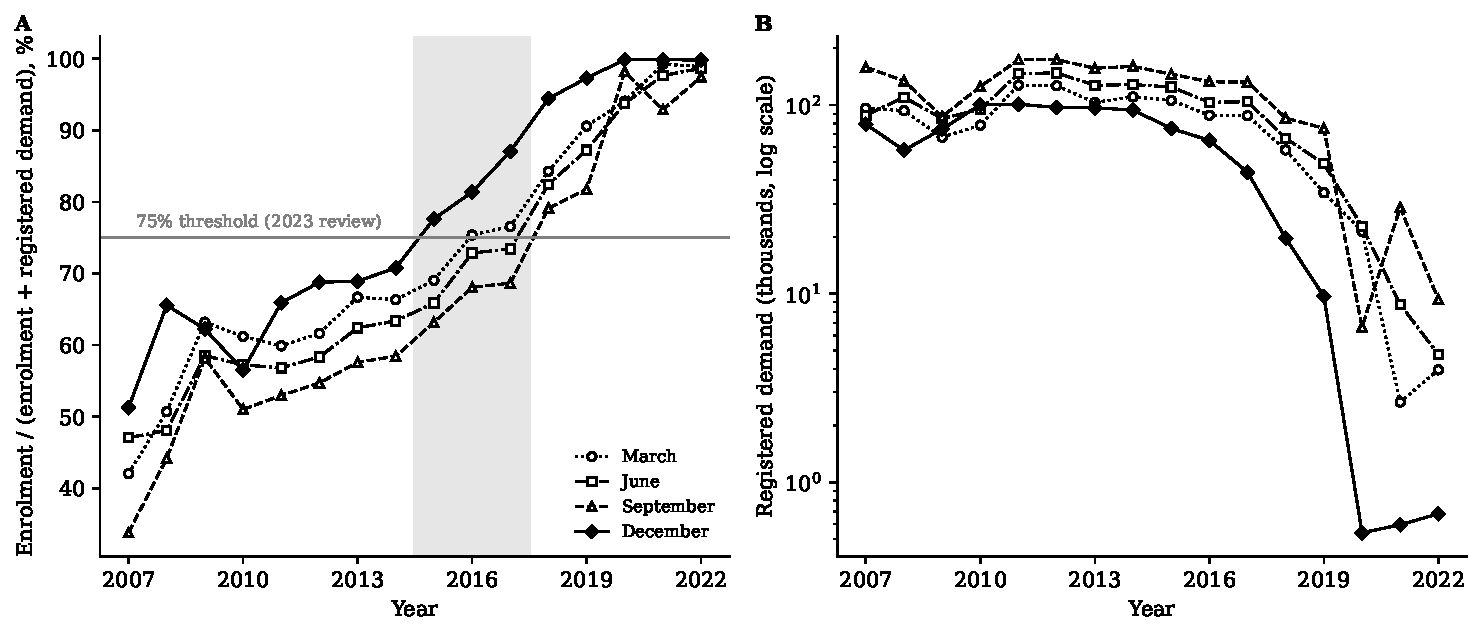
\includegraphics[width=\textwidth]{C_fig_goal}
\caption{Share of registered children served and registered demand in S\~ao Paulo, by reporting month, 2007--2022}
\label{fig:goal}
% Texto anterior, redigido com IA e fora de uso: _arquivo_texto_IA_2026-10-27/legendas_notas_corpo/V3w_fig_goal.tex
\tabnote{\emph{Sources:} Municipal Secretariat of Education (SME), published series of childcare enrolment and registered demand. Panel A reports childcare enrolment as a percentage of the sum of enrolment and registered demand. The horizontal line marks the 75\% threshold used in the 2023 review. The shaded interval identifies 2015--2017, when the December count met this threshold but the September count did not. Panel B reports registered demand in thousands of children on a logarithmic scale. Both panels distinguish the March, June, September and December counts, with the same series identification throughout. The series end in 2022, the last year for which all four counts are available. Registered demand measures recorded applications awaiting a place rather than the full population of children without access to childcare.}
\par\smallskip\noindent\begin{minipage}{\linewidth}\footnotesize\raggedright Alt text: Two-panel line chart covering 2007--2022, with four series corresponding to March, June, September and December observations. Panel A plots the percentage of registered children served, with a horizontal reference line at 75\% and shading over 2015--2017. Panel B plots registered demand in thousands of children on a logarithmic scale.\end{minipage}
\end{figure}

% Gerado por 02_audit/build15_tables.py (25/10/2026). Nao editar a mao.
\begin{table}[htbp]\centering
\caption{Coverage of the supplied request record among children entering childcare, 2010--2018}
\label{tab:coverage}
\footnotesize
\par\medskip\textbf{Panel A. Entrants in each year found in the request record}\par\smallskip
\fitbox{%
\begin{tabular}{lrrrrrrr}
\toprule
Year of entry & Entrants & In record (\%) & February (\%) & Other months (\%) & Centres & Median centre (share) & Centres $\geq$90\% (\%) \\
\midrule
2010 & 96,072 & 42.1 & 42.0 & 58.1 & 1,324 & 0.41 & 0.1 \\
2011 & 89,085 & 47.9 & 47.9 & 60.1 & 1,328 & 0.47 & 0.8 \\
2012 & 121,001 & 57.2 & 41.4 & 98.3 & 1,493 & 0.40 & 1.9 \\
2013 & 127,236 & 98.6 & 98.3 & 99.3 & 1,519 & 1.00 & 97.0 \\
2014 & 127,709 & 99.2 & 99.0 & 99.6 & 1,550 & 1.00 & 98.8 \\
2015 & 148,593 & 98.8 & 98.3 & 99.7 & 1,660 & 1.00 & 97.3 \\
2016 & 143,262 & 99.3 & 99.0 & 99.8 & 1,838 & 1.00 & 98.5 \\
2017 & 148,650 & 98.9 & 98.4 & 99.8 & 1,881 & 1.00 & 96.7 \\
2018 & 165,888 & 99.9 & 99.9 & 99.9 & 1,999 & 1.00 & 99.9 \\
\end{tabular}}
\par\medskip\textbf{Panel B. Share of each birth cohort enrolled before 24 months, by source (\% of live births)}\par\smallskip
\fitbox{%
\begin{tabular}{lrrr}
Birth cohort & Request record & Enrolment records & Difference \\
\midrule
2010 & 7.4 & 25.1 & $-$17.7 \\
2011 & 22.8 & 28.3 & $-$5.5 \\
2012 & 33.2 & 31.9 & +1.3 \\
2013 & 43.4 & 42.9 & +0.5 \\
2014 & 44.1 & 43.2 & +0.9 \\
2015 & 46.6 & 45.6 & +1.0 \\
2016 & 53.8 & 53.2 & +0.6 \\
\bottomrule
\end{tabular}}
% Texto anterior, redigido com IA e fora de uso: _arquivo_texto_IA_2026-10-27/legendas_notas_corpo/V2_coverage.tex
\tabnote{\emph{Sources:} SME childcare request record (applications dated 2010--2018, with referral and enrolment dates through November 2019); SME enrolment records (Escola On-Line, EOL). \emph{Sample:} children whose first childcare enrolment falls in each year from 2010 to 2018. \emph{Unit:} child. Coverage is the share of first entrants who can be matched to a first application in the supplied request files. It measures the completeness of the files available for this analysis, not necessarily that of SME's underlying administrative system. Figure~\ref{fig:coverage} presents the corresponding coverage measures by year of first enrolment, semester of first application and birth cohort.}
\end{table}

% FUSAO (26/10/2026): float copied unchanged from tables_C*.tex, tables_main.tex or tables_appendix.tex.
\begin{figure}[htbp]\centering
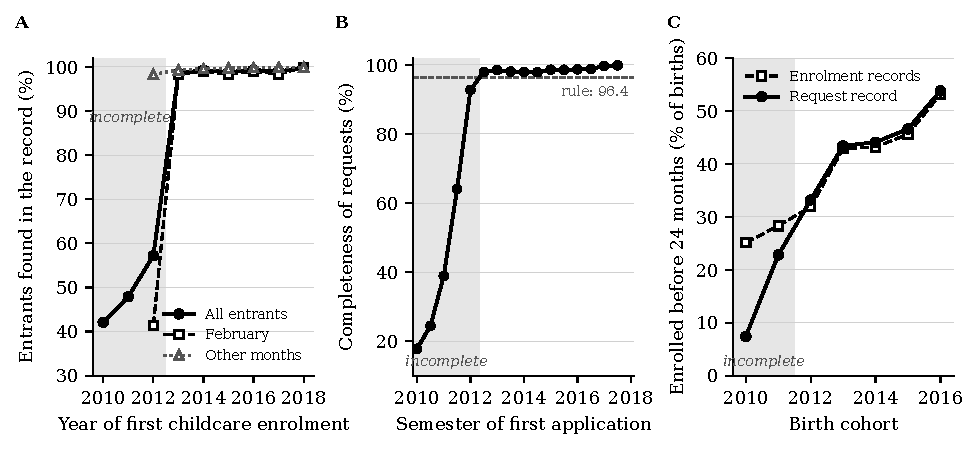
\includegraphics[width=\textwidth]{V3_fig_coverage}
\caption{Coverage of the childcare request records by enrolment year, application semester and birth cohort}
\label{fig:coverage}
% Texto anterior, redigido com IA e fora de uso: _arquivo_texto_IA_2026-10-27/legendas_notas_corpo/V3w_fig_coverage.tex
\tabnote{\emph{Sources:} SME childcare request records, enrolment records (EOL) and live birth registrations (SINASC). Panel A shows the percentage of children entering childcare for the first time between 2010 and 2018 whose applications can be identified in the supplied request records. The series distinguish all entrants, those first enrolled in February and those first enrolled in other months. The latter two series begin in 2012. Panel B reports estimated request-record completeness, calculated as $R/(R+M)$, by semester of first application from the first semester of 2010 to the second semester of 2017, where $M$ denotes imputed missing requests. The dashed line indicates the 96.4\% threshold used in the completeness rule. Panel C compares the percentage of each 2010--2016 birth cohort enrolled before 24 months of age according to the EOL and request records, using registered live births as the denominator. Shaded intervals indicate periods of incomplete record coverage. Differences between the series describe the coverage of the supplied records and do not establish the administrative reasons for missing observations.}
\par\smallskip\noindent\begin{minipage}{\linewidth}\footnotesize\raggedright Alt text: Three-panel chart of childcare request-record coverage. Panel A plots three annual series for the percentage of first-time entrants matched to request records from 2010 to 2018. Panel B plots estimated completeness by semester of first application, with a dashed reference line at 96.4\%, while Panel C compares two measures of enrolment before 24 months of age across the 2010--2016 birth cohorts. Shaded areas identify periods of incomplete coverage.\end{minipage}
\end{figure}



\clearpage
\appendix
\renewcommand{\thesection}{\Alph{section}}
\section{Supplementary tables and figures}
\label{sec:appendix-tables}
% Opening note of Appendix A: to be written by the author, if needed (the archived one stated the period convention of
% the tables from the request record; facts in ESQUELETO.md, section 6).
\setcounter{table}{0}\renewcommand{\thetable}{A\arabic{table}}
\setcounter{figure}{0}\renewcommand{\thefigure}{A\arabic{figure}}
\renewcommand{\theHtable}{A\arabic{table}}\renewcommand{\theHfigure}{A\arabic{figure}}
% tables_V3_appendix.tex -- generated by 02_audit/build12_order.py (FUSAO, 26/10/2026): floats in order of first citation. Do not edit by hand.
% Apendice A (revisao pos-EE). Gerado por 02_audit/build12_appendix.py; tabulars verbatim.
\begin{table}[htbp]\centering
\caption{Childcare classes at and above the module (authorized class size) by age band, 2016 and 2017}
\label{tab:T6a_modulo}
\footnotesize
\fitbox{%
\begin{tabular}{llrrrrr}
\toprule
Year & Age band & Classes & Module & Mean enrol. & \% at cap. & \% above \\
\midrule
2016 & Ber\c{c}\'ario I & 3,675 & 7 & 6.9 & 88.3 & 0.4 \\
2016 & Ber\c{c}\'ario II & 7,194 & 9 & 8.6 & 74.6 & 0.8 \\
2016 & Minigrupo I & 7,790 & 12 & 11.4 & 62.1 & 2.1 \\
2016 & Minigrupo II & 4,819 & 25 & 20.8 & 25.4 & 1.3 \\
2017 & Ber\c{c}\'ario I & 3,701 & 7 & 6.9 & 89.4 & 0.4 \\
2017 & Ber\c{c}\'ario II & 7,423 & 9 & 8.7 & 75.6 & 0.5 \\
2017 & Minigrupo I & 8,110 & 12 & 11.4 & 62.3 & 1.4 \\
2017 & Minigrupo II & 5,089 & 25 & 20.8 & 23.3 & 1.2 \\
\bottomrule
\end{tabular}}
\tabnote{\emph{Source:} municipal class profile (offered places, classes and enrolment by centre, age band and semester), 2013--2019. \emph{Sample:} childcare classes in 2016 and 2017. The module is the authorized class size, with modal values of 7, 9, 12 and 25 by age band. A class is ``at capacity'' when its enrolment equals the module and ``above'' when enrolment exceeds it. Entries are descriptive shares of classes.}
\end{table}

% Apendice A (revisao pos-EE). Gerado por 02_audit/build12_appendix.py; tabulars verbatim.
\begin{table}[htbp]\centering
\caption{Enrolment relative to authorized places, by age band and semester}
\label{tab:T6b_ratio}
\footnotesize
\fitbox{%
\begin{tabular}{lrrrrrrr}
\toprule
Age band & 2013S1 & 2014S1 & 2015S1 & 2016S1 & 2017S1 & 2018S1 & 2019S1 \\
\midrule
Ber\c{c}\'ario I & 0.994 & 0.994 & 0.992 & 0.993 & 0.994 & 0.929 & 0.977 \\
Ber\c{c}\'ario II & 0.993 & 0.994 & 0.981 & 0.993 & 0.996 & 0.959 & 0.989 \\
Minigrupo I & 0.988 & 0.992 & 0.992 & 0.991 & 0.994 & 0.970 & 0.986 \\
Minigrupo II & 0.974 & 0.979 & 0.992 & 0.992 & 0.988 & 0.980 & 0.984 \\
\bottomrule
\end{tabular}}
\tabnote{\emph{Source:} municipal class profile (offered places, classes and enrolment by centre, age band and semester), 2013--2019. \emph{Sample:} all childcare classes; 2018S1 is a mid-year snapshot, and second-semester columns are omitted. The ratio is total enrolment divided by total offered places. Enrolment enters only the numerator and never the definition of capacity. The ratios are descriptive.}
\end{table}

% Apendice A. Gerado por 02_audit/build15_appx.py (25/10/2026). Nao editar a mao.
\begin{table}[htbp]\centering
\caption{First requests, first referrals, and first enrolments by calendar month, 2013--2017 (column \%)}
\label{tab:calendar}
\footnotesize
\fitbox{%
\begin{tabular}{lrrr}
\toprule
Month & First applications & First referrals & First enrolments \\
\midrule
January & 10.0 & 7.1 & 15.1 \\
February & 15.9 & 8.7 & 12.5 \\
March & 9.6 & 8.2 & 9.4 \\
April & 7.3 & 4.9 & 5.5 \\
May & 6.9 & 3.8 & 4.6 \\
June & 6.3 & 2.9 & 3.1 \\
July & 6.6 & 2.3 & 2.6 \\
August & 8.8 & 3.4 & 3.6 \\
September & 7.6 & 2.9 & 3.1 \\
October & 7.6 & 2.8 & 2.7 \\
November & 8.5 & 2.5 & 2.3 \\
December & 5.0 & 50.5 & 35.5 \\
\addlinespace
N (events) & 881,957 & 918,624 & 788,082 \\
\bottomrule
\end{tabular}}
\tabnote{\emph{Source:} SME childcare request record (applications dated 2010--2018, with referral and enrolment dates through November 2019). \emph{Sample:} each child's first application, first referral and first enrolment, counted when the event falls in calendar years 2013--2017. Entries give the percentage of each type of event that falls in each calendar month, so columns sum to 100. The shares are descriptive.}
\end{table}

% Apendice A (revisao pos-EE). Gerado por 02_audit/build12_appendix.py; tabulars verbatim.
\begin{table}[htbp]\centering
\caption{Authorized childcare places, centres, and classes in municipal and contracted centres by age band and contractual mode, first semester of each year}
\label{tab:T2a_capacidade}
\label{tab:T2b_nescolas}
\label{tab:T2c_nturmas}
\footnotesize
\par\medskip\textbf{Panel A. Authorized places}\par\smallskip
\begin{tabular}{llrrrrrrr}
\toprule
Age band & Contractual mode & 2013S1 & 2014S1 & 2015S1 & 2016S1 & 2017S1 & 2018S1 & 2019S1 \\
\midrule
Ber\c{c}\'ario I & Direct & 4,016 & 4,203 & 4,133 & 3,836 & 3,822 & 3,540 & 3,710 \\
 & Partner & 15,717 & 17,340 & 20,904 & 21,862 & 21,844 & 26,334 & 28,910 \\
Ber\c{c}\'ario II & Direct & 11,850 & 11,878 & 10,498 & 10,764 & 11,619 & 11,725 & 12,823 \\
 & Partner & 35,555 & 40,560 & 41,130 & 52,107 & 52,835 & 63,195 & 73,579 \\
Minigrupo I & Direct & 19,896 & 20,035 & 18,020 & 18,467 & 18,476 & 19,240 & 18,174 \\
 & Partner & 53,251 & 56,984 & 58,197 & 71,527 & 74,552 & 85,638 & 85,866 \\
Minigrupo II & Direct & 20,850 & 21,870 & 23,900 & 24,221 & 23,309 & 23,331 & 22,272 \\
 & Partner & 53,426 & 52,050 & 66,359 & 77,167 & 83,836 & 91,019 & 93,559 \\
\end{tabular}
\par\medskip\textbf{Panel B. Centres with at least one childcare class}\par\smallskip
\begin{tabular}{llrrrrrrr}
Age band & Contractual mode & 2013S1 & 2014S1 & 2015S1 & 2016S1 & 2017S1 & 2018S1 & 2019S1 \\
\midrule
Ber\c{c}\'ario I & Direct & 238 & 239 & 228 & 222 & 222 & 213 & 230 \\
 & Partner & 742 & 779 & 897 & 997 & 1,033 & 1,147 & 1,267 \\
Ber\c{c}\'ario II & Direct & 346 & 347 & 342 & 344 & 353 & 358 & 369 \\
 & Partner & 1,059 & 1,139 & 1,242 & 1,480 & 1,535 & 1,716 & 1,888 \\
Minigrupo I & Direct & 366 & 369 & 368 & 369 & 374 & 377 & 381 \\
 & Partner & 1,179 & 1,246 & 1,360 & 1,600 & 1,665 & 1,824 & 1,923 \\
Minigrupo II & Direct & 415 & 433 & 423 & 416 & 396 & 400 & 395 \\
 & Partner & 1,143 & 1,121 & 1,264 & 1,500 & 1,582 & 1,703 & 1,821 \\
\end{tabular}
\par\medskip\textbf{Panel C. Childcare classes}\par\smallskip
\begin{tabular}{llrrrrrrr}
Age band & Contractual mode & 2013S1 & 2014S1 & 2015S1 & 2016S1 & 2017S1 & 2018S1 & 2019S1 \\
\midrule
Ber\c{c}\'ario I & Direct & 582 & 608 & 598 & 556 & 552 & 515 & 541 \\
 & Partner & 2,255 & 2,495 & 3,015 & 3,153 & 3,150 & 3,802 & 4,175 \\
Ber\c{c}\'ario II & Direct & 1,345 & 1,355 & 1,199 & 1,230 & 1,328 & 1,348 & 1,492 \\
 & Partner & 4,051 & 4,639 & 4,718 & 6,009 & 6,087 & 7,281 & 8,480 \\
Minigrupo I & Direct & 1,745 & 1,762 & 1,591 & 1,641 & 1,644 & 1,721 & 1,644 \\
 & Partner & 4,580 & 4,909 & 5,032 & 6,216 & 6,483 & 7,411 & 7,467 \\
Minigrupo II & Direct & 1,009 & 1,046 & 1,167 & 1,192 & 1,141 & 1,148 & 1,107 \\
 & Partner & 2,539 & 2,450 & 3,147 & 3,644 & 3,948 & 4,247 & 4,368 \\
\bottomrule
\end{tabular}
\tabnote{\emph{Source:} municipal class profile (offered places, classes and enrolment by centre, age band and semester), 2013--2019. \emph{Sample:} all municipal and contracted childcare centres in the first semester of each year; 2018S1 is a June snapshot, and second-semester columns are omitted. ``Direct'' denotes municipally operated centres. In this table, ``Partner'' covers the whole contracted network, combining partner-run and indirect centres, which are distinguished in Section~\ref{sec:institutions} and Table~\ref{tab:T5c_modal}. Authorized places are offered places, and no measure in the table uses enrolment. Entries are descriptive totals.}
\end{table}

% Apendice A (revisao pos-EE). Gerado por 02_audit/build12_appendix.py; tabulars verbatim.
\begin{table}[htbp]\centering
\caption{Authorized capacity measured by offered places and by classes times the statutory module}
\label{tab:R_capcheck}
\footnotesize
\fitbox{%
\begin{tabular}{lrrrrrr}
\toprule
& \multicolumn{3}{c}{Offered places} & \multicolumn{3}{c}{Classes $\times$ statutory module} \\
\cmidrule(lr){2-4}\cmidrule(lr){5-7}
Age band & 2013S1 & 2019S1 & Change \% & 2013S1 & 2019S1 & Change \% \\
\midrule
Ber\c{c}\'ario I & 19,733 & 32,620 & 65.3 & 19,859 & 33,012 & 66.2 \\
Ber\c{c}\'ario II & 47,405 & 86,402 & 82.3 & 48,564 & 89,748 & 84.8 \\
Minigrupo I & 73,147 & 104,040 & 42.2 & 75,900 & 109,332 & 44.0 \\
Minigrupo II & 74,276 & 115,831 & 55.9 & 88,700 & 136,875 & 54.3 \\
\addlinespace
Total & 214,561 & 338,893 & 57.9 & 233,023 & 368,967 & 58.3 \\
\bottomrule
\end{tabular}}
\tabnote{\emph{Source:} municipal class profile (offered places, classes and enrolment by centre, age band and semester), 2013--2019. \emph{Sample:} first semesters of 2013 and 2019. The table compares the growth of two measures of authorized capacity: offered places, and the number of classes multiplied by the statutory module of the age band (7, 9, 12 or 25). The second measure is built only from class counts and statutory modules, so it is independent of enrolment by construction. Across band-semester cells, the ratio of offered places to module-based capacity lies between 0.837 and 0.994. The comparison is descriptive.}
\end{table}

% FUSAO (26/10/2026): float copied unchanged from tables_C*.tex, tables_main.tex or tables_appendix.tex.
\begin{figure}[htbp]\centering
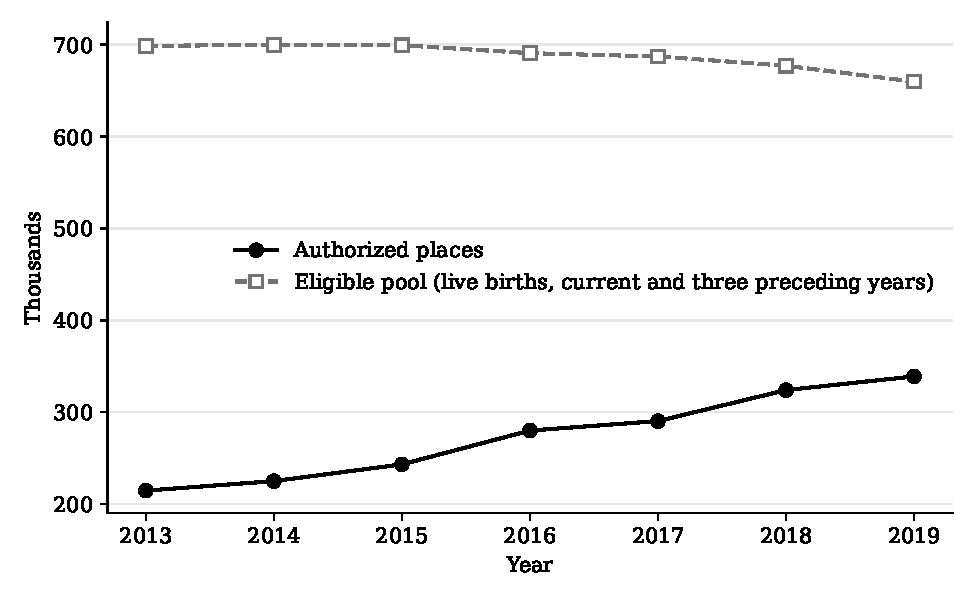
\includegraphics[width=0.85\textwidth]{F7_capacidade_pool}
\caption{Authorized childcare places in the first semester and the eligible population based on annual live births, S\~ao Paulo, 2013--2019}
\label{fig:F7}
\tabnote{\emph{Sources:} Municipal class profile (authorized places, first semester); SINASC live births. Authorized places refer to the first semester of each year. The eligible population is calculated as the sum of live births in the reference calendar year and the preceding three years. It is not scaled to Census counts and therefore differs from the population series in Table~\ref{tab:arms}. Both series are shown as descriptive levels, expressed in thousands.}
\par\smallskip\noindent\begin{minipage}{\linewidth}\footnotesize\raggedright Alt text: Line chart comparing two annual series, measured in thousands, from 2013 to 2019. One series shows authorized childcare places in the first semester of each year; the other shows the eligible population calculated from live births in that year and the three preceding years.\end{minipage}
\end{figure}

% Apendice A (revisao pos-EE). Gerado por 02_audit/build12_appendix.py; tabulars verbatim.
\begin{table}[htbp]\centering
\caption{Centres with at least one childcare class in the first-semester profile, by contractual mode}
\label{tab:T7a_ceis}
\footnotesize
\begin{tabular}{lrrrrrrr}
\toprule
Contractual mode & 2013 & 2014 & 2015 & 2016 & 2017 & 2018 & 2019 \\
\midrule
Direct & 418 & 447 & 435 & 426 & 406 & 414 & 402 \\
Partner & 1,223 & 1,287 & 1,395 & 1,642 & 1,696 & 1,870 & 2,004 \\
Total & 1,641 & 1,734 & 1,830 & 2,068 & 2,102 & 2,284 & 2,406 \\
\bottomrule
\end{tabular}
\tabnote{\emph{Source:} municipal class profile (offered places, classes and enrolment by centre, age band and semester), 2013--2019. \emph{Sample:} centres with at least one childcare class in the first-semester profile. ``Direct'' denotes municipally operated centres. In this table, ``Partner'' covers the whole contracted network, combining partner-run and indirect centres, which are distinguished in Section~\ref{sec:institutions} and Table~\ref{tab:T5c_modal}. Entries are descriptive counts of centres.}
\end{table}

% Apendice A (revisao pos-EE). Gerado por 02_audit/build12_appendix.py; tabulars verbatim.
\begin{table}[htbp]\centering
\caption{Authorized places per eligible child and the decomposition of its change, 2013--2019}
\label{tab:S6c_cobertura}
\label{tab:S6d_decomp}
\footnotesize
\par\medskip\textbf{Panel A. Places per eligible child}\par\smallskip
\begin{tabular}{lrrrrr}
\toprule
Year & Capacity (mun.) & Pool 0--3 (mun.) & Per child (mun.) & Per child Q1 & Per child Q4 \\
\midrule
2013 & 214,561 & 698,781 & 0.307 & 0.377 & 0.175 \\
2014 & 224,920 & 699,958 & 0.321 & 0.391 & 0.174 \\
2015 & 243,141 & 699,479 & 0.348 & 0.426 & 0.182 \\
2016 & 279,951 & 690,805 & 0.405 & 0.495 & 0.196 \\
2017 & 290,293 & 687,234 & 0.422 & 0.521 & 0.201 \\
2018 & 324,022 & 677,171 & 0.478 & 0.574 & 0.226 \\
2019 & 338,893 & 659,818 & 0.514 & 0.615 & 0.252 \\
\end{tabular}
\par\medskip\textbf{Panel B. Decomposition of the 2013--2019 change}\par\smallskip
\begin{tabular}{lrr}
Component & Value (places per child) & \% of gain \\
\midrule
Total gain 2013--2019 & 0.207 & 100 \\
\addlinespace
Capacity growth & 0.178 & 86 \\
Pool 0--3 contraction & 0.029 & 14 \\
\bottomrule
\end{tabular}
\tabnote{\emph{Sources:} municipal class profile (offered places, classes and enrolment by centre, age band and semester), 2013--2019; live births by district of residence from the municipal health secretariat's vital statistics (SINASC). \emph{Unit and period:} S\~ao Paulo municipality and district income quartiles, first semesters of 2013--2019. The eligible pool in year $Y$ is the sum of live births in $Y$, $Y-1$, $Y-2$ and $Y-3$, and places per eligible child are first-semester authorized places divided by that pool. Panel B decomposes the 2013--2019 change, holding the pool at its 2013 level to obtain the capacity component and capacity at its 2019 level to obtain the pool component. The decomposition is descriptive, and the split between the two components depends on this order.}
\end{table}

% Apendice A (revisao pos-EE). Gerado por 02_audit/build12_appendix.py; tabulars verbatim.
\begin{table}[htbp]\centering
\caption{Enrolled children by the centre's contractual mode and year of enrolment (row \%)}
\label{tab:T5c_modal}
\footnotesize
\begin{tabular}{lrrr}
\toprule
Year & Direct & Indirect & Partner \\
\midrule
2010 & 23.9 & 24.8 & 51.3 \\
2011 & 27.0 & 23.8 & 49.2 \\
2012 & 23.9 & 24.5 & 51.6 \\
2013 & 21.5 & 23.9 & 54.6 \\
2014 & 19.2 & 21.8 & 59.0 \\
2015 & 17.4 & 18.0 & 64.6 \\
2016 & 16.9 & 18.6 & 64.4 \\
2017 & 15.3 & 18.0 & 66.8 \\
2018 & 13.9 & 16.4 & 69.7 \\
\bottomrule
\end{tabular}
\tabnote{\emph{Source:} SME childcare request record (applications dated 2010--2018, with referral and enrolment dates through November 2019). \emph{Sample:} enrolled children, by year of enrolment. Children are classified by the contractual mode of the centre of enrolment (direct, indirect or partner), and rows sum to 100. The shares are descriptive.}
\end{table}

% Apendice A (revisao pos-EE). Gerado por 02_audit/build12_appendix.py; tabulars verbatim.
\begin{table}[htbp]\centering
\caption{Characteristics of first requests by request year, including postcode income, enrolment within 365 days, and children never enrolled}
\label{tab:T1_fila}
\footnotesize
\fitbox{%
\begin{tabular}{lrrrrrr}
\toprule
Characteristic & 2010 & 2012 & 2014 & 2016 & 2018 & Total \\
\midrule
N applications & 81,004 & 220,922 & 174,676 & 172,341 & 165,331 & 1,524,560 \\
\% female & 49.1 & 49.0 & 48.7 & 49.0 & 48.5 & 48.8 \\
\% White & 36.3 & 33.4 & 29.7 & 29.0 & 33.9 & 31.9 \\
\% Black & 2.6 & 2.7 & 2.5 & 2.7 & 2.9 & 2.7 \\
\% Brown & 24.5 & 24.4 & 23.7 & 23.2 & 27.6 & 24.5 \\
\% Asian & 0.3 & 0.3 & 0.3 & 0.4 & 0.5 & 0.3 \\
\% Indigenous & 0.2 & 0.2 & 0.2 & 0.3 & 0.3 & 0.2 \\
\% Other/NA & 36.1 & 39.2 & 43.5 & 44.4 & 34.9 & 40.4 \\
Median age at application (months) & 35 & 23 & 15 & 12 & 11 & 16 \\
\% with priority & 3.7 & 11.1 & 18.9 & 20.4 & 15.0 & 14.5 \\
Median postcode income (R\$) & 927 & 939 & 940 & 943 & 947 & 939 \\
Median N of centres $\leq$2\,km & 33 & 33 & 32 & 32 & 31 & 32 \\
\% enrolled within 365d & 52.2 & 61.3 & 63.0 & 69.7 & 80.7 & 64.5 \\
\% never enrolled & 29.2 & 12.1 & 9.6 & 8.6 & 18.3 & 13.4 \\
\bottomrule
\end{tabular}}
\tabnote{\emph{Source:} SME childcare request record (applications dated 2010--2018, with referral and enrolment dates through November 2019). \emph{Sample:} first application per child (1,524,560). The Total column includes 51,106 applications from 2006--2009, and odd years are omitted for space. Postcode income is the mean household income of the census tract. ``Enrolled within 365 days'' and ``never enrolled'' both refer to enrolment in any municipal centre before the end of the panel. Entries are descriptive shares and medians.}
\end{table}

% Apendice A (revisao pos-EE). Gerado por 02_audit/build12_appendix.py; tabulars verbatim.
\begin{table}[htbp]\centering
\caption{First applications sharing the same timestamp to the second, by year of application}
\label{tab:N1}
\footnotesize
\fitbox{%
\begin{tabular}{lrrrrr}
\toprule
Year of application & N & $\geq$2 & $\geq$10 & $\geq$50 & $\geq$100 \\
\midrule
2010 & 81,004 & 1.7 & 0.1 & 0.0 & 0.0 \\
2011 & 124,240 & 1.8 & 0.0 & 0.0 & 0.0 \\
2012 & 220,922 & 3.0 & 0.0 & 0.0 & 0.0 \\
2013 & 191,149 & 2.4 & 0.0 & 0.0 & 0.0 \\
2014 & 174,676 & 2.7 & 0.0 & 0.0 & 0.0 \\
2015 & 179,869 & 2.9 & 0.6 & 0.6 & 0.6 \\
2016 & 172,341 & 2.5 & 0.0 & 0.0 & 0.0 \\
2017 & 163,922 & 2.7 & 0.0 & 0.0 & 0.0 \\
2018 & 165,331 & 2.7 & 0.0 & 0.0 & 0.0 \\
\addlinespace
Total & 1,524,560 & 2.7 & 0.1 & 0.1 & 0.1 \\
\bottomrule
\end{tabular}}
\tabnote{\emph{Source:} SME childcare request record (applications dated 2010--2018, with referral and enrolment dates through November 2019). \emph{Sample:} first application per child (1,524,560, including 51,106 first applications dated 2006--2009 that are not shown by year). Timestamps are recorded to the second. For $k = 2, 10, 50, 100$, entries give the share of first applications whose timestamp is shared by at least $k$ first applications made anywhere in the city in that second. The shares are descriptive.}
\end{table}

% FUSAO (26/10/2026): NEW. Body generated by 02_audit/build22_robustez.py (robustness item 1 of the triage).
\begin{table}[htbp]\centering
\caption{Arm~A of Goal~5 under the main population series and three alternatives, S\~ao Paulo, 2010--2024}
\label{tab:armArob}
% Gerado por 02_audit/build22_robustez.py (FUSAO, 26/10/2026). Nao editar a mao.
\footnotesize
\setlength{\tabcolsep}{4pt}
\fitbox{%
\begin{tabular}{l rrr rrrr rr c}
\toprule
 & \multicolumn{3}{c}{Population 0--3 (000)} & \multicolumn{4}{c}{Stage enrolment, per cent of population} & \multicolumn{2}{c}{Age, per cent} & Binding arm \\
\cmidrule(lr){2-4}\cmidrule(lr){5-8}\cmidrule(lr){9-10}
Year & SEADE & Censuses & Births & SEADE & Censuses & Censuses, linear & Births & SEADE & Censuses & (Censuses) \\
\midrule
2010 & 570 & 564 & 693 & 30.0 & 30.3 & 30.3 & 24.6 & 38.3 & 38.7 & A \\
2011 & 569 & 564 & 695 & 43.3 & 43.6 & 44.3 & 35.4 & 37.6 & 37.9 & A \\
2012 & 568 & 566 & 699 & 46.3 & 46.4 & 48.0 & 37.6 & 40.3 & 40.5 & A \\
2013 & 566 & 564 & 700 & 47.2 & 47.4 & 49.6 & 38.2 & 44.8 & 45.0 & A \\
2014 & 565 & 563 & 700 & 49.9 & 50.2 & 53.1 & 40.3 & 47.5 & 47.7 & A \\
2015 & 564 & 561 & 701 & 52.9 & 53.2 & 57.1 & 42.6 & 50.7 & 50.9 & A \\
2016 & 561 & 557 & 697 & 59.0 & 59.4 & 64.3 & 47.4 & 56.5 & 57.0 & A \\
2017 & 558 & 550 & 691 & 61.5 & 62.5 & 67.8 & 49.7 & 58.6 & 59.5 & A \\
2018 & 556 & 543 & 684 & 65.8 & 67.4 & 73.5 & 53.5 & 62.9 & 64.5 & A \\
2019 & 553 & 530 & 671 & 70.0 & 73.0 & 79.1 & 57.7 & 66.8 & 69.7 & A \\
2020 & 550 & 514 & 652 & 69.2 & 74.1 & 79.1 & 58.4 & 65.6 & 70.3 & A \\
2021 & 541 & 492 & 627 & 69.8 & 76.8 & 79.9 & 60.3 & 65.7 & 72.3 & B \\
2022 & 532 & 465 & 594 & 73.3 & 83.8 & 83.8 & 65.6 & 68.7 & 78.6 & B \\
2023 & 523 & -- & 562 & 72.1 & -- & -- & 67.0 & 67.6 & -- & -- \\
2024 & 513 & -- & 534 & 72.2 & -- & -- & 69.5 & 67.8 & -- & -- \\
\bottomrule
\end{tabular}}

\tabnote{\emph{Sources:} Inep school census; IBGE Population Censuses of 2010 and 2022; SINASC live births; SEADE population projections. \emph{Population aged zero to three} (thousands): the SEADE series interpolates linearly between the projections published for 2010, 2015, 2020 and 2025 \citep{seade_idade_escolar}. The main series, ``Censuses'' (as in Table~\ref{tab:arms}), is built for the May school census of each year $Y$. Live births to residents from June of $Y-4$ to May of $Y$, the birth months of children aged zero to three at that census, are divided by the ratio of this births pool to the Census count of children aged zero to three; the ratio is interpolated linearly between 2010 (1.228) and 2022 (1.278), so the series equals the Census count in 2010 (564{,}210) and in 2022 (464{,}826) \citep{ibge_sidra1378,ibge_sidra9514}. ``Censuses, linear'' interpolates in a straight line between the two Census counts, and ``Births'' is the births pool without Census scaling. No Census-based value is reported after 2022. \emph{Enrolment:} May school census \citep{inep_censo_escolar_c}; ``Stage'' is childcare-stage enrolment in all networks, and ``Age'' counts enrolled children aged zero to three in any stage. \emph{Binding arm (Censuses):} the arm requiring more children to be served in December under the Censuses denominator, with Arm~A equal to 75\% of the population and Arm~B to municipal enrolment plus registered demand (Table~\ref{tab:series}). The comparison is descriptive.}
\end{table}

% RETOMADA (27/10/2026), decision D2: all 144 combinations of the choices the law leaves open. Body generated by
% 02_audit/build25_indeterminacia.py with 02_audit/build25_tabelas.py (C_indet_full_body.tex); every combination and
% year is in 03_build/build25/combinacoes.csv.
\begin{table}[htbp]\centering
\caption{Years in which Goal~5 is met under the 144 specifications of our measurement grid, S\~ao Paulo, 2010--2022}
\label{tab:indetfull}
\fitbox{% Gerado por 02_audit/build25_indeterminacia.py com 02_audit/build25_tabelas.py (RETOMADA, 27/10/2026). Nao editar a mao.
\footnotesize
\setlength{\tabcolsep}{4pt}
\begin{tabular}{l l l l l l l l}
\toprule
 & Enrolment in & \multicolumn{3}{c}{Arm A on all networks} & \multicolumn{3}{c}{Arm A on municipal and partner centres} \\
\cmidrule(lr){3-5}\cmidrule(lr){6-8}
Population series & Arm B & Dec. & Sep. & Mean & Dec. & Sep. & Mean \\
\midrule
\multicolumn{8}{l}{\textbf{Panel A. Only the greater arm must be met}} \\
\multicolumn{8}{l}{\emph{Published list (all requests)}} \\
\quad Births scaled to Censuses & Secretariat & never & never & never & never & never & never \\
\quad  & School census & 2021 & never & 2021 & never & never & never \\
\quad Straight line between Censuses & Secretariat & 2019 & never & never & never & never & never \\
\quad  & School census & 2019--2021 & 2020 & 2020 & never & never & never \\
\quad SEADE projection & Secretariat & never & never & never & never & never & never \\
\quad  & School census & never & never & never & never & never & never \\
\addlinespace
\multicolumn{8}{l}{\emph{Narrower list (no specific-centre requests)}} \\
\quad Births scaled to Censuses & Secretariat & 2021--2022 & never & never & 2021 & never & never \\
\quad  & School census & 2021 & never & 2021 & never & never & never \\
\quad Straight line between Censuses & Secretariat & 2019--2022 & never & never & 2020--2021 & never & never \\
\quad  & School census & 2019--2021 & 2020 & 2020--2021 & never & never & never \\
\quad SEADE projection & Secretariat & never & never & never & never & never & never \\
\quad  & School census & never & never & never & never & never & never \\
\addlinespace
\multicolumn{8}{l}{\textbf{Panel B. An empty list is required whichever arm is greater}} \\
\multicolumn{8}{l}{\emph{Published list (all requests)}} \\
\quad Births scaled to Censuses & Secretariat & never & never & never & never & never & never \\
\quad  & School census & never & never & never & never & never & never \\
\quad Straight line between Censuses & Secretariat & never & never & never & never & never & never \\
\quad  & School census & never & never & never & never & never & never \\
\quad SEADE projection & Secretariat & never & never & never & never & never & never \\
\quad  & School census & never & never & never & never & never & never \\
\addlinespace
\multicolumn{8}{l}{\emph{Narrower list (no specific-centre requests)}} \\
\quad Births scaled to Censuses & Secretariat & 2021--2022 & never & never & 2021 & never & never \\
\quad  & School census & 2021 & never & never & never & never & never \\
\quad Straight line between Censuses & Secretariat & 2020--2022 & never & never & 2020--2021 & never & never \\
\quad  & School census & 2020--2021 & never & never & never & never & never \\
\quad SEADE projection & Secretariat & never & never & never & never & never & never \\
\quad  & School census & never & never & never & never & never & never \\
\addlinespace
\multicolumn{8}{l}{\textbf{Panel C. All 144 combinations}} \\
\multicolumn{7}{l}{\quad Goal never met in an evaluable year} & 123 \\
\multicolumn{7}{l}{\quad Goal met in at least one year} & 21 \\
\multicolumn{7}{l}{\qquad first met in 2019} & 4 \\
\multicolumn{7}{l}{\qquad first met in 2020} & 8 \\
\multicolumn{7}{l}{\qquad first met in 2021} & 9 \\
\multicolumn{7}{l}{\qquad of which: met in one year and not in a later evaluable year} & 4 \\
\multicolumn{7}{l}{\quad Goal met in any year before 2019} & 0 \\
\multicolumn{7}{l}{\quad Distinct sets of years in which the goal is met} & 9 \\
\bottomrule
\end{tabular}
}
\tabnote{\emph{Sources:} as in Table~\ref{tab:indet}. \emph{Specifications:} the goal, its arms and the measurement choices are defined as in Table~\ref{tab:indet}, which reproduces the December column of Panel~A for Arm~A on all networks, including the rows based on SEADE's population projection \citep{seade_idade_escolar}. This table retains all the count dates the law leaves open: December, September, and the mean of the year's four quarterly counts. SME Ordinance 7{,}972 later fixed December 31 for recording the indicator; the December publications used here are not all extracted on that date (Table~\ref{tab:dates}). It also adds two readings not included in Table~\ref{tab:indet} (Section~\ref{sec:goal}): Arm~A counted on municipal and partner centres only, whose census fields are usable through 2021; and an empty waiting list required whichever arm is greater, with Arm~A also required when it is the greater one (Panel~B). \emph{Entries:} the years in which each specification meets the goal; ``never'' indicates that the goal is met in no year in which the specification can be computed. A specification is computable only in years in which all its inputs exist: 2019--2022 on the narrower list (2020--2022 for its annual mean), through 2021 on census enrolment or with Arm~A on municipal and partner centres, and 2010--2022 otherwise. Of the 21 specifications that meet the goal, 14 do so only in 2020--2021, and none of these 14 can be computed for 2022 (Section~\ref{sec:pandemic}). The classifications are descriptive.}
\end{table}

% FUSAO (26/10/2026): float copied unchanged from tables_C*.tex, tables_main.tex or tables_appendix.tex.
\begin{table}[htbp]\centering
\caption{Waiting list reconstructed from the request record as a share of the published list, end of quarter, 2010--2018}
\label{tab:recon}
% Gerado por 02_audit/build20_tables.py (26/10/2026). Nao editar a mao.
\footnotesize
\fitbox{%
\begin{tabular}{lrrrr}
\toprule
Year & March & June & September & December \\
\midrule
2010 & 0.33 & 0.25 & 0.20 & 0.31 \\
2011 & 0.31 & 0.32 & 0.35 & 0.85 \\
2012 & 0.92 & 0.92 & 0.91 & 0.83 \\
2013 & 0.96 & 0.94 & 0.93 & 0.91 \\
2014 & 0.96 & 0.93 & 0.91 & 0.87 \\
2015 & 0.94 & 0.91 & 0.89 & 0.88 \\
2016 & 0.93 & 0.92 & 0.89 & 0.92 \\
2017 & 0.95 & 0.93 & 0.92 & 0.94 \\
2018 & 0.95 & 0.93 & 0.90 & 0.95 \\
\bottomrule
\end{tabular}}

\tabnote{\emph{Sources:} SME childcare request record (applications dated 2010--2018, with referral dates through November 2019); SME publications of registered demand (Table~\ref{tab:series}). \emph{Unit and period:} S\~ao Paulo municipality, quarter ends, 2010--2018. The reconstructed list counts children younger than 47 months whose first request is dated on or before the last day of the quarter and who, by that day, have neither been referred nor had a withdrawal recorded. Each entry divides this count by published registered demand for the same month. Requests in the supplied extract end in December 2018, so 2019 is not shown. The ratios describe the coverage of the supplied files.}
\end{table}

% FUSAO (26/10/2026): NEW. Body generated by 02_audit/build22_robustez.py (robustness item 2 of the triage).
\begin{table}[htbp]\centering
\caption{Entries to and exits from the reconstructed waiting list between the end of September and the end of December, 2013--2018}
\label{tab:decomp}
% Gerado por 02_audit/build22_robustez.py (FUSAO, 26/10/2026). Nao editar a mao.
\footnotesize
\fitbox{%
\begin{tabular}{l r r rrr r r}
\toprule
 & List on & New & \multicolumn{3}{c}{Left the list} & List on & December referrals made \\
\cmidrule(lr){4-6}
Year & 30 Sep. & requests & Referred & Aged out & Withdrew & 31 Dec. & by extraction date (\%) \\
\midrule
2013 & 145{,}627 & 32{,}395 & 86{,}418 & 3{,}301 & 257 & 88{,}046 & -- \\
2014 & 146{,}161 & 30{,}969 & 91{,}364 & 3{,}348 & 229 & 82{,}189 & 100.0 \\
2015 & 130{,}343 & 37{,}853 & 98{,}605 & 3{,}265 & 201 & 66{,}125 & 100.0 \\
2016 & 118{,}722 & 29{,}468 & 86{,}165 & 1{,}860 & 255 & 59{,}910 & 100.0 \\
2017 & 121{,}478 & 30{,}065 & 108{,}760 & 1{,}091 & 449 & 41{,}243 & 99.2 \\
2018 & 77{,}247 & 31{,}097 & 89{,}034 & 372 & 318 & 18{,}620 & 99.8 \\
\bottomrule
\end{tabular}}

\tabnote{\emph{Sources:} SME childcare request record (applications dated 2010--2018, with referral dates through November 2019); extraction dates printed on SME's December publications (Table~\ref{tab:dates}). \emph{Unit and period:} S\~ao Paulo municipality, September 30 to December 31 of each year, 2013--2018. The list is reconstructed as in Table~\ref{tab:recon}: children younger than 47 months with a first request on file, not referred and with no recorded withdrawal. ``New requests'' are first requests made between October 1 and December 31. ``Left the list'' counts children whose first exit from the list in that period is a referral, reaching 47 months without referral, or a recorded withdrawal. The list on September 30 plus new requests minus exits equals the list on December 31 exactly. The last column gives the share of referrals dated in December that were made on or before the extraction date printed on that year's December publication; no December 2013 publication is posted. All entries are descriptive.}
\end{table}

% FUSAO (26/10/2026): float copied unchanged from tables_C*.tex, tables_main.tex or tables_appendix.tex.
\begin{table}[htbp]\centering
\caption{Extraction dates printed on the December publications of registered demand}
\label{tab:dates}
% Gerado por 02_audit/build20_tables.py (26/10/2026). Nao editar a mao.
\footnotesize
\fitbox{%
\begin{tabular}{lll}
\toprule
Year & Extraction date printed & Note \\
\midrule
2007 & 31 December 2007 &  \\
2008 & 31 December 2008 &  \\
2009 & 31 December 2009 &  \\
2010 & 31 December 2010 &  \\
2011 & 31 December 2011 &  \\
2012 & 27 December 2012 &  \\
2014 & 31 December 2014 &  \\
2015 & 31 December 2015 &  \\
2016 & 31 December 2016 &  \\
2017 & 28 December 2017 &  \\
2018 & 27 December 2018 &  \\
2019 & 31 December 2019 &  \\
2020 & 9 December 2020 &  \\
2021 & 8 December 2021 & marked ``Ajustado'' (adjusted) \\
2022 & 30 November 2022 &  \\
2023 & 25 December 2023 &  \\
2024 & 31 December 2024 &  \\
2025 & 18 December 2025 &  \\
\bottomrule
\end{tabular}}

\tabnote{\emph{Source:} SME publications of enrolment and registered demand, PDF files, with the date taken from the footer ``Sistema EOL - [date]'' \citep{sme_demanda_escolar}. No December 2013 publication is posted. Entries are transcribed from the publications.}
\end{table}

% Apendice A. Gerado por 02_audit/build15_appx.py (25/10/2026). Nao editar a mao.
\begin{table}[htbp]\centering
\caption{Percentage of children first enrolled in February who have a request in the request record, by year and centre type, for types with at least 200 February entrants in 2012}
\label{tab:covtype}
\footnotesize
\fitbox{%
\begin{tabular}{lrrrrrrrr}
\toprule
Type of centre & 2011 & 2012 & 2013 & 2014 & N 2011 & N 2012 & N 2013 & N 2014 \\
\midrule
CEI DIRET & 45.4 & 39.2 & 98.8 & 99.5 & 14,602 & 18,184 & 18,783 & 17,736 \\
CEI INDIR & 48.9 & 39.8 & 98.6 & 99.2 & 19,984 & 18,856 & 22,666 & 23,110 \\
CEU CEI & 39.4 & 35.7 & 98.5 & 99.4 & 3,023 & 4,804 & 5,100 & 4,611 \\
CEU EMEI & -- & 32.0 & 95.8 & 98.3 & -- & 610 & 120 & 115 \\
CR.P.CONV & 48.7 & 43.6 & 98.0 & 98.8 & 51,182 & 40,148 & 44,711 & 44,884 \\
EMEI & -- & 42.6 & 96.7 & 97.3 & -- & 4,529 & 1,374 & 1,290 \\
\bottomrule
\end{tabular}}
\tabnote{\emph{Sources:} SME childcare request record (applications dated 2010--2018, with referral and enrolment dates through November 2019); SME enrolment records (EOL). \emph{Sample:} children whose first childcare enrolment is dated in February of each year, in centre types with at least 200 February entrants in 2012. Entries give the percentage of entrants with a first request in the request record. Centre types are those recorded in the enrolment records: CEI DIRET (direct), CEI INDIR (indirect), CR.P.CONV (partner), CEU (unified education centres) and EMEI (preschool units with childcare classes). The shares are descriptive.}
\end{table}

% Gerado por 02_audit/build18_tables.py (26/10/2026). Nao editar a mao.
\begin{table}[htbp]\centering
\caption{Completeness of the request record by request semester, children first enrolled in 2010--2018}
\label{tab:completeness}
\footnotesize
\par\medskip\textbf{Panel A. By semester of first application}\par\smallskip
\fitbox{%
\begin{tabular}{lrrrrc}
\toprule
Semester & \shortstack[r]{Entrants with a\\prior request} & \shortstack[r]{Entrants without one,\\assigned} & \shortstack[r]{Completeness\\(\%)} & \shortstack[r]{Referral\\recorded (\%)} & \shortstack[c]{Meets\\the rule} \\
\midrule
2010S1 & 8,332 & 38,404 & 17.8 & 70.0 & no \\
2010S2 & 11,005 & 34,040 & 24.4 & 76.2 & no \\
2011S1 & 20,357 & 32,034 & 38.9 & 97.1 & no \\
2011S2 & 39,635 & 22,245 & 64.1 & 99.4 & no \\
2012S1 & 72,920 & 5,652 & 92.8 & 99.4 & no \\
2012S2 & 55,300 & 1,135 & 98.0 & 99.3 & yes \\
2013S1 & 69,831 & 1,046 & 98.5 & 99.5 & yes \\
2013S2 & 55,283 & 1,051 & 98.1 & 99.2 & yes \\
2014S1 & 67,060 & 1,447 & 97.9 & 99.2 & yes \\
2014S2 & 59,289 & 1,278 & 97.9 & 99.1 & yes \\
2015S1 & 73,067 & 1,051 & 98.6 & 99.5 & yes \\
2015S2 & 66,048 & 962 & 98.6 & 99.6 & yes \\
2016S1 & 77,776 & 1,034 & 98.7 & 99.6 & yes \\
2016S2 & 59,319 & 737 & 98.8 & 99.6 & yes \\
2017S1 & 72,305 & 205 & 99.7 & 99.8 & yes \\
2017S2 & 51,833 & 64 & 99.9 & 99.9 & yes \\
\end{tabular}}
\par\medskip\textbf{Panel B. By birth cohort}\par\smallskip
\fitbox{%
\begin{tabular}{lrrr}
Birth cohort & Applicants & Applications before July 2012 (\%) & Completeness, weighted (\%) \\
\midrule
2010 & 128,352 & 47.6 & 82.8 \\
2011 & 146,693 & 35.6 & 92.0 \\
2012 & 155,292 & 8.2 & 97.9 \\
2013 & 153,033 & 0.0 & 98.4 \\
2014 & 151,772 & 0.0 & 98.6 \\
2015 & 146,293 & 0.0 & 99.0 \\
2016 & 128,143 & 0.0 & 99.4 \\
\bottomrule
\end{tabular}}
\tabnote{\emph{Sources:} SME childcare request record (applications dated 2010--2018, with referral and enrolment dates through November 2019); SME enrolment records (EOL), first childcare enrolment per child, entries 2010--2018. \emph{Sample:} children whose first childcare enrolment falls in 2010--2018. ``Entrants with a prior request'' are children whose first recorded request falls in the semester and precedes their first enrolment. ``Entrants without one'' have no request recorded before their first enrolment; they are distributed across the semesters in which they would have applied, using the distribution of the time from request to entry among 2014--2017 entrants with a request, estimated separately for February and other months (medians of 314 and 232 days). Completeness is the first group divided by the sum of both. ``Referral recorded'' is the percentage of the semester's applicants who entered care after applying and have a referral recorded in the request record within 60 days after entry. Panel B weights semester completeness by the semester distribution of each cohort's first applications. Under a rule fixed before the computation, a semester is complete if both completeness and referral recording fall no more than two percentage points below their 2014S1--2016S2 means (thresholds of 96.4\% and 97.4\%). With the lag distribution of 2014 entrants only, or of 2016--2017 entrants only, completeness is 92.6--93.3\% in 2012S1 and 97.9--98.1\% in 2012S2. The exercise is descriptive and assumes that children absent from the record had the same lag as those present.}
\end{table}

% Gerado por 02_audit/build18_appx.py (26/10/2026). Nao editar a mao.
\begin{table}[htbp]\centering
\caption{Is the request record prospective? Timing of requests relative to entry, and outcomes that a record created at enrolment would not contain}
\label{tab:prospect}
\footnotesize
\par\medskip\textbf{Panel A. Entrants by year of first childcare enrolment}\par\smallskip
\fitbox{%
\begin{tabular}{lrrrrrr}
\toprule
Year of entry & Entrants & \shortstack[r]{In record\\(\%)} & \shortstack[r]{Median days,\\request to entry} & \shortstack[r]{Request after\\entry (\%)} & \shortstack[r]{Request 0--7 days\\before entry (\%)} & \shortstack[r]{Request $>$30 days\\before entry (\%)} \\
\midrule
2012 & 121,001 & 57.2 & 12 & 36.54 & 10.2 & 43.7 \\
2013 & 127,236 & 98.6 & 324 & 0.64 & 5.5 & 89.5 \\
2014 & 127,709 & 99.2 & 320 & 0.41 & 4.0 & 92.1 \\
2015 & 148,593 & 98.8 & 307 & 1.01 & 4.1 & 90.7 \\
2016 & 143,262 & 99.3 & 252 & 0.49 & 2.3 & 91.8 \\
2017 & 148,650 & 98.9 & 274 & 0.58 & 2.7 & 93.0 \\
2018 & 165,888 & 99.9 & 214 & 0.00 & 5.5 & 88.4 \\
\end{tabular}}
\par\medskip\textbf{Panel B. Applicants by year of first application}\par\smallskip
\fitbox{%
\begin{tabular}{lrrrrrr}
\shortstack[r]{Year of\\application} & Applicants & \shortstack[r]{Never\\enrolled (\%)} & \shortstack[r]{Never in care,\\EOL (\%)} & \shortstack[r]{Recorded\\refusal (\%)} & \shortstack[r]{Centre never\\attended (\%)} & \shortstack[r]{Centre not\\requested (\%)} \\
\midrule
2012 & 220,922 & 12.1 & 28.4 & 31.1 & 24.9 & 51.1 \\
2013 & 191,149 & 10.3 & 24.8 & 33.2 & 27.5 & 57.3 \\
2014 & 174,676 & 9.6 & 22.5 & 33.9 & 29.4 & 65.3 \\
2015 & 179,869 & 7.9 & 19.1 & 34.4 & 30.7 & 75.6 \\
2016 & 172,341 & 8.6 & 18.5 & 32.0 & 29.4 & 79.7 \\
2017 & 163,922 & 9.3 & 16.8 & 29.9 & 28.5 & 80.9 \\
\bottomrule
\end{tabular}}
\tabnote{\emph{Sources:} SME childcare request record (applications dated 2010--2018, with referral and enrolment dates through November 2019); SME enrolment records (EOL), first childcare enrolment per child. \emph{Samples:} Panel A, children by year of first childcare enrolment, with the percentage columns after the second computed among those found in the record; Panel B, children by year of first application. Days to entry run from the first recorded request to the first enrolment. ``Request after entry'' means that the first request is dated after the first enrolment, and ``0--7 days'' that the request precedes entry by at most seven days, the same day included. ``Never enrolled'' indicates no enrolment in the request record by November 2019; ``never in care'' indicates no childcare enrolment in EOL. ``Recorded refusal'' indicates at least one recorded refusal, and ``centre never attended'' at least one referral to a centre where the child never enrolled. ``Centre not requested'' is the percentage of referral rows whose centre differs from the one requested. Before 2012, EOL dates almost every entry to the start of the school year, so Panel A starts in 2012. The shares are descriptive.}
\end{table}

% FUSAO (26/10/2026): float copied unchanged from tables_C*.tex, tables_main.tex or tables_appendix.tex.
\begin{figure}[htbp]\centering
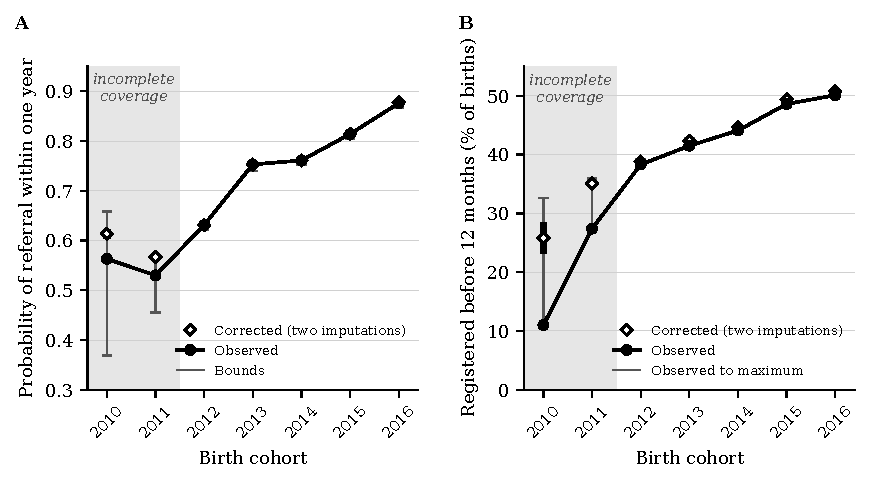
\includegraphics[width=0.95\textwidth]{V3_fig_level}
\caption{Observed and corrected levels by birth cohort for a service measure and a count}
\label{fig:level}
\tabnote{\emph{Sources:} SME childcare request record (applications dated 2010--2018, with referral dates through November 2019); SME enrolment records (EOL), entries through December 2018; SINASC live births. \emph{Sample:} applicants with eligible time in each birth cohort, plus the cohort's entrants with no request recorded before entry. Panel A shows referral within 365 days of the first application; Panel B shows children registered before 12 months as a percentage of live births. Circles are levels observed in the request record. Thick bars and diamonds show the corrected level as the range and midpoint of two imputations, defined in the note to Table~\ref{tab:level}. Thin lines show the bounds in Panel A and the range from the observed level to the maximum in Panel B. Shaded cohorts have applications partly in semesters of incomplete coverage. The figure is descriptive; Table~\ref{tab:level} reports the values for the 2010--2013 and 2016 cohorts.}
\par\smallskip\noindent\begin{minipage}{\linewidth}\footnotesize\raggedright Alt text: Two-panel chart organized by birth cohort from 2010 to 2016. Each panel displays observed estimates as circles and corrected estimates as diamonds with thick uncertainty bars. Thin lines indicate the corresponding bounds across cohorts.\end{minipage}
\end{figure}

% Apendice A (Fase 2): copia da antiga tabela do corpo, agora leitura do extrato completo. Origem: N4_enrolled.tex
% BUILD12. Descritivo. Gerado por 02_audit/build12_tables.py.
\begin{table}[htbp]\centering
\caption{Share of each birth cohort enrolled and registered by a given age, full extract}
\label{tab:enrolledbyage}
\footnotesize
\setlength{\tabcolsep}{4pt}
\fitbox{%
\begin{tabular}{lrrrrrr}
\toprule
 & & \multicolumn{3}{c}{Enrolled before (\% of births)} & \multicolumn{2}{c}{Registered before (\% of births)} \\
\cmidrule(lr){3-5}\cmidrule(lr){6-7}
Birth cohort & Live births & 12 months & 24 months & 36 months & 12 months & 24 months \\
\midrule
2010 & 174,116 & 1.9 & 7.4 & 30.7 & 11.0 & 33.7 \\
2011 & 176,268 & 2.1 & 22.8 & 44.0 & 27.4 & 50.3 \\
2012 & 175,679 & 11.6 & 33.2 & 52.5 & 38.3 & 59.4 \\
2013 & 172,718 & 13.2 & 43.4 & 60.7 & 41.5 & 62.3 \\
2014 & 175,293 & 15.0 & 44.1 & 62.7 & 44.1 & 66.3 \\
2015 & 175,789 & 20.8 & 46.6 & 68.6 & 48.6 & 69.4 \\
2016 & 167,005 & 22.7 & 53.8 &  & 50.1 & 70.9 \\
2017 & 169,147 & 25.1 &  &  & 50.9 &  \\
\bottomrule
\end{tabular}
}
\tabnote{\emph{Sources:} SME childcare request record (first application and enrolment dates); live births by year from the municipal vital statistics (SINASC/CEInfo). \emph{Sample:} birth cohorts 2010--2017; a cell is reported only if the whole cohort reaches the stated age within the panel. The numerator counts children of the cohort first enrolled in municipal childcare, or first registered, before the stated age; the denominator is live births in the municipality in the birth year. Because the two sources are not linked at the child level, the levels are approximate. Unlike the registered stock, these flows are indexed to the child's age and do not depend on when the snapshot is taken. The shares are descriptive.}
\end{table}

% Gerado por 02_audit/build18_tables.py (26/10/2026). Nao editar a mao.
\begin{table}[htbp]\centering
\caption{Observed and corrected levels for birth cohorts with incomplete coverage}
\label{tab:level}
\footnotesize
\par\medskip\textbf{Panel A. Level of each statistic, by birth cohort}\par\smallskip
\fitbox{%
\begin{tabular}{llrrrrr}
\toprule
Statistic & & 2010 & 2011 & 2012 & 2013 & 2016 \\
\midrule
Missing entrants & N (\% of applicants) & 39,022 (36.7) & 15,825 (12.5) & 1,761 (1.3) & 2,240 (1.6) & 1,227 (1.0) \\
\addlinespace[0.6em]
One-year referral & Observed & 0.563 & 0.530 & 0.631 & 0.753 & 0.876 \\
 & Bounds & [0.369, 0.658] & [0.455, 0.570] & [0.622, 0.635] & [0.740, 0.756] & [0.868, 0.878] \\
 & Corrected & 0.605--0.622 & 0.566--0.567 & 0.631 & 0.752--0.753 & 0.878 \\
\addlinespace[0.6em]
One-year enrolment & Observed & 0.468 & 0.427 & 0.523 & 0.644 & 0.747 \\
 & Bounds & [0.299, 0.589] & [0.363, 0.478] & [0.516, 0.528] & [0.633, 0.649] & [0.740, 0.750] \\
 & Corrected & 0.521--0.545 & 0.469--0.473 & 0.524 & 0.644--0.645 & 0.749 \\
\addlinespace[0.6em]
Registered $<$12m (\% births) & Observed & 11.0 & 27.4 & 38.3 & 41.5 & 50.1 \\
 & Maximum & 32.6 & 35.9 & 39.2 & 42.7 & 50.8 \\
 & Corrected & 23.2--28.4 & 34.6--35.6 & 38.8 & 42.3 & 50.8 \\
\addlinespace[0.6em]
Enrolled $<$24m (\% births) & Request record & 7.4 & 22.8 & 33.2 & 43.4 & 53.8 \\
 & Enrolment records & 25.1 & 28.3 & 31.9 & 42.9 & 53.2 \\
\end{tabular}}
\par\medskip\textbf{Panel B. Change over the cohorts and the part due to coverage}\par\smallskip
\fitbox{%
\begin{tabular}{llrrrrr}
Measure & Cohorts & Observed & Corrected & Bounds on the & \multicolumn{2}{c}{Coverage share (\%)} \\
 & & change & change & corrected change & estimate & bounds \\
\midrule
One-year referral & 2010--2016 & 0.313 & 0.256--0.273 & [0.218, 0.507] & 13--18 & $-$62 to 30 \\
One-year enrolment & 2010--2016 & 0.279 & 0.204--0.228 & [0.158, 0.448] & 18--27 & $-$61 to 43 \\
Registered $<$12m (\% births) & 2010--2016 & 39.1 & 22.4--27.6 & [17.5, 39.1] & 29--43 & 0 to 55 \\
Enrolled $<$24m (\% births) & 2010--2016 & 46.4 & 28.1 & -- & 39 & -- \\
\addlinespace[0.6em]
One-year referral & 2012--2016 & 0.245 & 0.247 & [0.241, 0.254] & $-$1 & -- \\
Registered $<$12m (\% births) & 2012--2016 & 11.8 & 12.0 & [10.9, 11.8] & $-$2 & -- \\
Enrolled $<$24m (\% births) & 2012--2016 & 20.6 & 21.3 & -- & $-$3 & -- \\
\bottomrule
\end{tabular}}
\tabnote{\emph{Sources:} SME childcare request record (applications dated 2010--2018, with referral and enrolment dates through November 2019); SME enrolment records (EOL), first childcare enrolment per child, entries through December 2018; SINASC live births. \emph{Sample:} applicants with eligible time in each birth cohort (N), plus missing entrants, that is, children of the cohort who entered childcare at 0--47 months with no request recorded before entry. Missing entrants with a later request are removed from N and counted once, as missing. Outcomes are referral and enrolment within 365 days of the first application, and registration before 12 months and enrolment before 24 months as percentages of live births. The lower and upper bounds assume that no missing entrant or every missing entrant, respectively, had the outcome; ``Maximum'' assumes that every missing entrant registered before 12 months. For the corrected levels, each missing entrant receives the mean outcome of entrants with a request in the same cell of age at entry (in months) and entry month (February or other), computed either from 2014--2017 entrants or from entrants of the same year; the reported range spans the two. In an out-of-sample check on 2013 entrants, the 2014--2017 reference gives 48.1\% against 46.5\% registered before 12 months, 69.3\% against 67.0\% referred within a year, and 62.7\% against 61.8\% enrolled within a year. In Panel B, the bounds on the corrected change hold the 2016 cohort at its observed level, and the coverage share is (observed $-$ corrected)/observed; for enrolment before 24 months, the corrected change is the change in the enrolment records. The exercise is descriptive, and the corrected levels assume that missing entrants resemble entrants with a request in the same cell.}
\end{table}

% Gerado por 02_audit/build18_tables.py (26/10/2026). Nao editar a mao.
\begin{table}[htbp]\centering
\caption{Timing of registration in the window of complete coverage}
\label{tab:timing}
\footnotesize
\fitbox{%
\begin{tabular}{lrrrrrrr}
\toprule
Birth cohort & Live births & $<$6m & $<$12m & $<$24m & $<$12m among $<$24m & 2010 district mix & 2016 district mix \\
\midrule
2012 & 175,679 & 23.5 & 38.3 & 59.4 & 0.644 & 0.643 & 0.643 \\
2013 & 172,718 & 26.1 & 41.5 & 62.3 & 0.666 & 0.666 & 0.666 \\
2014 & 175,293 & 28.1 & 44.1 & 66.3 & 0.664 & 0.665 & 0.664 \\
2015 & 175,789 & 31.4 & 48.6 & 69.4 & 0.701 & 0.702 & 0.701 \\
2016 & 167,005 & 33.4 & 50.1 & 70.9 & 0.707 & 0.708 & 0.707 \\
\bottomrule
\end{tabular}}
\tabnote{\emph{Sources:} SME childcare request record (applications dated 2010--2018, with referral and enrolment dates through November 2019); live births by district of residence (SINASC). \emph{Sample:} birth cohorts 2012--2016, each observed from birth to 24 months. The $<$6m, $<$12m and $<$24m columns give children with a first application before each age as a percentage of live births. The $<$12m among $<$24m column is the share registered before 12 months among children registered before 24 months. The last two columns average district-specific shares, weighting districts by the composition of the 2010 or the 2016 cohort. Between the 2012 and 2016 cohorts, the share registered before 12 months among those registered before 24 months rose in 93 of 96 districts (median within-district change +0.060; range $-$0.023 to +0.252). The shares are descriptive.}
\end{table}

% FUSAO (26/10/2026): float copied unchanged from tables_C*.tex, tables_main.tex or tables_appendix.tex.
\begin{figure}[htbp]\centering
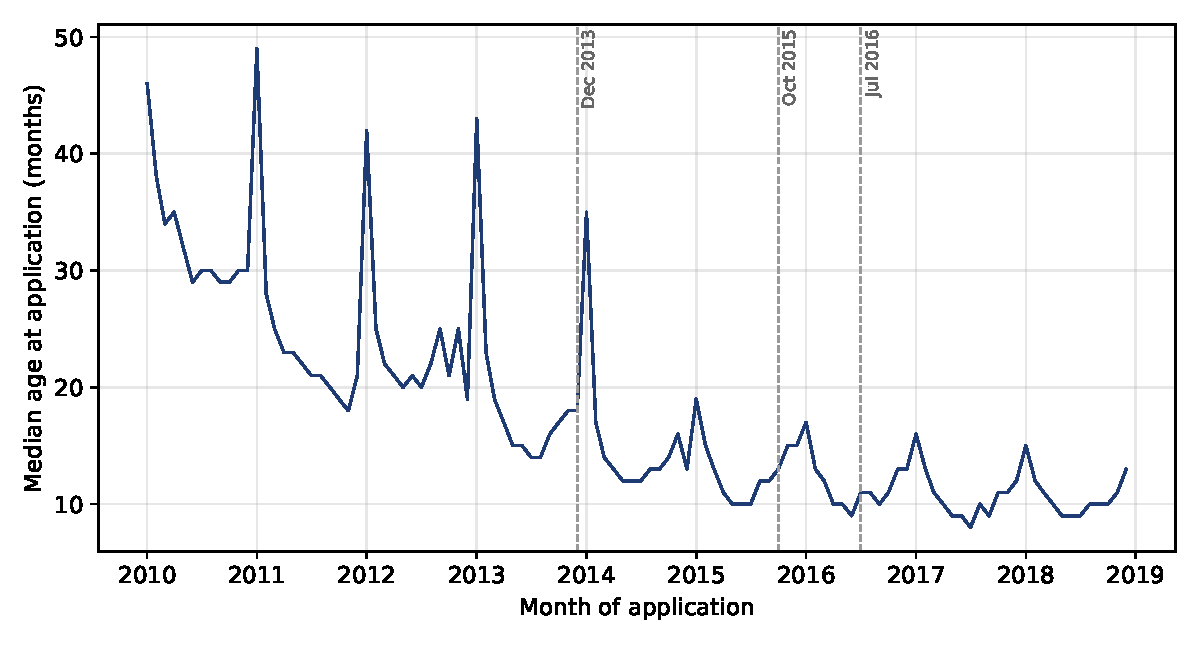
\includegraphics[width=0.85\textwidth]{F8_serie_mensal}
\caption{Median age at first application by month of application, full extract, January 2010 to December 2018}
\label{fig:F8}
\tabnote{\emph{Source:} SME childcare request record. \emph{Sample:} first application per child, by calendar month, January 2010 to December 2018. The series is the monthly median age at first application, in months. Dashed lines mark December 2013, October 2015 and July 2016. The October 2015 and July 2016 lines correspond to ordinances on enrolment rules and automated matching. The December 2013 line is kept only as a visual reference, because the date of the change that introduced socioeconomic priority has not been verified. The figure is descriptive.}
\par\smallskip\noindent\begin{minipage}{\linewidth}\footnotesize\raggedright Alt text: Monthly time-series chart showing the median age at first childcare application from January 2010 to December 2018. Three dashed vertical lines mark reference dates along the series.\end{minipage}
\end{figure}

% Apendice A. Gerado por 02_audit/build15_appx.py (25/10/2026). Nao editar a mao.
\begin{table}[htbp]\centering
\caption{Enrolment and repeat referral among referred children by age at request and days to first referral, first requests 2013--2018}
\label{tab:C4}
\footnotesize
\fitbox{%
\begin{tabular}{llrrrr}
\toprule
Age at application & Referral speed & N & Enrolment rate \% & Median age at enr. & Re-ref.\ \% \\
\midrule
0--5m & 0--30d & 22,935 & 94.3 & 4 & 87.2 \\
0--5m & 31--90d & 39,239 & 93.0 & 5 & 77.2 \\
0--5m & 91--180d & 75,191 & 93.8 & 7 & 75.2 \\
0--5m & $>$180d & 171,950 & 93.5 & 13 & 71.4 \\
6--11m & 0--30d & 15,447 & 94.6 & 9 & 86.6 \\
6--11m & 31--90d & 18,650 & 91.4 & 11 & 76.6 \\
6--11m & 91--180d & 30,720 & 91.4 & 13 & 73.1 \\
6--11m & $>$180d & 102,544 & 91.0 & 20 & 68.7 \\
12--23m & 0--30d & 27,641 & 93.0 & 19 & 83.8 \\
12--23m & 31--90d & 26,557 & 90.0 & 20 & 74.3 \\
12--23m & 91--180d & 39,580 & 89.2 & 21 & 71.0 \\
12--23m & $>$180d & 123,860 & 87.8 & 29 & 64.2 \\
24m+ & 0--30d & 153,214 & 93.6 & 49 & 78.8 \\
24m+ & 31--90d & 52,636 & 90.7 & 46 & 72.1 \\
24m+ & 91--180d & 44,005 & 88.0 & 42 & 67.6 \\
24m+ & $>$180d & 82,975 & 84.6 & 46 & 58.1 \\
\bottomrule
\end{tabular}}
\tabnote{\emph{Source:} SME childcare request record (applications dated 2010--2018, with referral and enrolment dates through November 2019). \emph{Sample:} referred children whose first application is dated 2013 or later. Referral speed is the number of days from application to first referral. The enrolment rate is the percentage enrolled at or after the first referral, and median age at enrolment is given in months. Re-referral is the percentage referred again among children with a recorded formal refusal. Entries are descriptive cell shares.}
\end{table}

% Gerado por 02_audit/build18_tables.py (26/10/2026). Nao editar a mao.
\begin{table}[htbp]\centering
\caption{Referral and enrolment within one year in the window of complete coverage among requesters with eligible time, 2012--2016 cohorts (Panel A) and 2013--2017 requests (Panel B)}
\label{tab:service}
\footnotesize
\par\medskip\textbf{Panel A. By birth cohort}\par\smallskip
\fitbox{%
\begin{tabular}{lrrrrrrrrr}
\toprule
Birth cohort & N & ref$_{180}$ & ref$_{365}$ & ref$_{730}$ & age$_{365}$ & RMST$_{365}$ & Median & enr$_{365}$ & RMST enr. \\
\midrule
2012 & 139,440 & 0.314 & 0.631 & 0.902 & 0.036 & 237 & 287 & 0.523 & 260 \\
2013 & 140,811 & 0.417 & 0.753 & 0.945 & 0.023 & 203 & 223 & 0.644 & 230 \\
2014 & 146,665 & 0.392 & 0.761 & 0.971 & 0.009 & 215 & 233 & 0.639 & 244 \\
2015 & 146,232 & 0.472 & 0.814 & 0.982 & 0.002 & 195 & 194 & 0.686 & 230 \\
2016 & 128,143 & 0.522 & 0.876 & 0.993 & 0.000 & 181 & 171 & 0.747 & 220 \\
\end{tabular}}
\par\medskip\textbf{Panel B. By calendar year of application}\par\smallskip
\fitbox{%
\begin{tabular}{lrrrr}
Year of application & N & ref$_{365}$ & enr$_{365}$ & Median \\
\midrule
2013 & 154,924 & 0.646 & 0.551 & 278 \\
2014 & 149,412 & 0.684 & 0.583 & 262 \\
2015 & 157,525 & 0.786 & 0.666 & 203 \\
2016 & 154,623 & 0.767 & 0.654 & 196 \\
2017 & 148,267 & 0.903 & 0.764 & 187 \\
\end{tabular}}
\par\medskip\textbf{Panel C. By semester of application, before and after the July 2016 allocation ordinance}\par\smallskip
\fitbox{%
\begin{tabular}{lrrr}
Semester of application & N & ref$_{365}$ & enr$_{365}$ \\
\midrule
2012S2 & 73,630 & 0.562 & 0.465 \\
2013S1 & 87,365 & 0.707 & 0.611 \\
2013S2 & 67,559 & 0.568 & 0.474 \\
2014S1 & 80,344 & 0.739 & 0.638 \\
2014S2 & 69,068 & 0.620 & 0.519 \\
2015S1 & 82,977 & 0.810 & 0.691 \\
2015S2 & 74,548 & 0.760 & 0.639 \\
2016S1 & 87,782 & 0.800 & 0.682 \\
2016S2 & 66,841 & 0.724 & 0.616 \\
2017S1 & 83,849 & 0.916 & 0.765 \\
2017S2 & 64,418 & 0.887 & 0.762 \\
2018S1 & 85,583 & 0.974 & 0.821 \\
\bottomrule
\end{tabular}}
\tabnote{\emph{Source:} SME childcare request record (applications dated 2010--2018, with referral and enrolment dates through November 2019). \emph{Sample:} applicants with eligible time (first application at or before 47 months). Panel A covers the 2012--2016 birth cohorts; Panel B, first applications in calendar years 2013--2017 (the window begins in July 2012, so 2013 is its first full year); and Panel C, the semesters 2012S2--2018S1, since later applications lack 365 days of follow-up. Time is counted in days from the first application. The ref$_{t}$ columns give the cumulative incidence of referral by day $t$; age$_{365}$ is the cumulative incidence of ageing out (reaching 47 months without referral) by day 365; RMST is the restricted mean number of days without the event within 365 days; Median is the day on which referral incidence reaches 0.5; and enr denotes the same measures with enrolment as the terminal event. In Panel C, semesters from 2016S2 onward fall after the ordinance of July 14, 2016, which formalized automated matching. Incidences are Aalen--Johansen estimates with ageing out as the competing event and are descriptive.}
\end{table}

% Gerado por 02_audit/build18_tables.py (26/10/2026). Nao editar a mao.
\begin{table}[htbp]\centering
\caption{Gain in one-year referral between the 2012 and 2016 cohorts under alternative specifications, including two that move the start of the window of complete coverage}
\label{tab:specs}
\footnotesize
\fitbox{%
\begin{tabular}{lrrrl}
\toprule
Specification & 2012 & 2016 & $\Delta$ & Interval or range \\
\midrule
Base: referral, ageing out competing & 0.631 & 0.876 & +0.245 & -- \\
Recorded withdrawal as a further competing event & 0.628 & 0.872 & +0.244 & -- \\
Children who applied after 47 months counted as ageing out & 0.571 & 0.876 & +0.305 & -- \\
Applications in the first calendar semester only & 0.694 & 0.911 & +0.217 & -- \\
Applications dated July 2012--December 2013 excluded & 0.730 & 0.876 & +0.146 & -- \\
2012 cohort restricted to applications from July 2012 & 0.607 & 0.876 & +0.269 & -- \\
Enrolment as the terminal event & 0.523 & 0.747 & +0.224 & -- \\
Composition held at 2012 (main cells) & 0.631 & 0.891 & +0.259 & [+0.256, +0.262] \\
Composition held at 2012, coarse / fine cells & -- & -- & +0.257 / +0.250 & -- \\
Composition and service environment held fixed & 0.631 & 0.869 & +0.238 & coarse +0.249, fine +0.238 \\
Unweighted, bootstrap interval & 0.631 & 0.876 & +0.245 & [+0.242, +0.249] \\
\addlinespace
\multicolumn{5}{l}{\emph{Specifications that move the start of the window}} \\
Window starting with the 2013 cohort & 0.753 & 0.876 & +0.123 & -- \\
Window starting with the 2014 cohort & 0.761 & 0.876 & +0.115 & -- \\
\bottomrule
\end{tabular}}
\tabnote{\emph{Source:} SME childcare request record (applications dated 2010--2018, with referral and enrolment dates through November 2019). \emph{Sample:} applicants with eligible time in the 2012--2016 birth cohorts, except where a row states otherwise; the last two rows move the start of the window and report the change from the 2013 or the 2014 cohort. The outcome is the cumulative incidence of referral (or enrolment) within 365 days of the first application, estimated with the Aalen--Johansen estimator; $\Delta$ is computed from unrounded incidences. Reweighted specifications match the 2012 cohort's joint distribution of applicant attributes. The main cells combine age at application, priority, postcode-income quartile, district and semester; the coarse cells use age, priority and income; the fine cells use eight age bins, priority, income, district and month. Weights are trimmed at the 1st and 99th percentiles. The service-environment specification adds the number of centres open within 2\,km at the application date. Intervals are percentile intervals from 1,000 bootstrap replications that resample children within the 2012 and 2016 cohorts and recompute the weights in each replication (seed 20260726); they reflect sampling variability only. In the exact decomposition of the raw change, composition contributes $-$0.014 and the service environment +0.022, leaving +0.238. All estimates are descriptive.}
\end{table}

% Apendice A. Gerado por 02_audit/build15_appx.py (25/10/2026). Nao editar a mao.
\begin{table}[htbp]\centering
\caption{Children who never enrolled compared with children who enrolled, first requests 2013--2017 (881,957 children)}
\label{tab:T4d_never}
\footnotesize
\fitbox{%
\begin{tabular}{lrr}
\toprule
Variable & Never enrolled & Enrolled \\
\midrule
N & 80,534 & 801,423 \\
Age at application (months) & 26.0 & 19.6 \\
With legal priority (\%) & 4.7 & 19.2 \\
Postcode income (R\$) & 1,367 & 1,207 \\
\bottomrule
\end{tabular}}
\tabnote{\emph{Source:} SME childcare request record (applications dated 2010--2018, with referral and enrolment dates through November 2019). \emph{Sample:} first applications dated 2013--2017 (881,957 children). A child is ``never enrolled'' if no enrolment in a municipal centre is recorded before the end of the panel. Postcode income is the mean household income of the census tract (2010 Census). Entries are descriptive group means. Because the groups differ by construction in age at application and priority, the differences between them are partly mechanical.}
\end{table}

% FUSAO (26/10/2026): float copied unchanged from tables_C*.tex, tables_main.tex or tables_appendix.tex.
\begin{table}[htbp]\centering
\caption{Change between 2014 and 2017 in the waiting-list stock and in flow measures, by the month in which the count or window ends}
\label{tab:stab}
% Gerado por 02_audit/build20_tables.py (26/10/2026). Nao editar a mao.
\footnotesize
\fitbox{%
\begin{tabular}{lrrrrr}
\toprule
Measure, change 2014 to 2017 & March & June & September & December & Dec./Sep. \\
\midrule
Registered demand, snapshot at month end (\%) & $-$20.5 & $-$18.9 & $-$17.5 & $-$53.2 & 3.03 \\
New first requests, 12 months to month end (\%) & $-$8.3 & $-$5.4 & $-$8.2 & $-$6.2 & 0.75 \\
Median age at first request, same window (months) & $-$5.2 & $-$4.6 & $-$4.1 & $-$3.8 & 0.93 \\
Referred within 365 days, same window (share) & $+$0.130 & $+$0.146 & $+$0.172 & $+$0.191 & 1.11 \\
\bottomrule
\end{tabular}}

\tabnote{\emph{Sources:} SME publications (registered demand); SME childcare request record, first requests from July 2012, with referral dates through November 2019 (flow measures). \emph{Unit:} S\~ao Paulo municipality. Registered demand is the count in the publication for the stated month (December extraction dates in Table~\ref{tab:dates}; the September 2017 publication prints no extraction date). New first requests, median age at first request and the share of first requests referred within 365 days are measured over the twelve months ending in the stated month. Entries are changes between the 2014 and 2017 values, in per cent for registered demand and new requests, in months for median age, and as a change in the share for referral. Dec./Sep.\ denotes the change measured in December divided by the change measured in September. The comparison starts in 2014 because March 2014 is the first March whose preceding twelve-month window lies wholly inside the window of complete coverage; over 2013--2017, the stock ratio is 3.47. The referral share is the simple share of all first requests in each window referred within 365 days, without the competing-event treatment, so its level differs from that in Table~\ref{tab:service}. Part of the contrast between the stock and the flows is mechanical: the stock is a count on a single day, whereas the flow measures cover twelve months. The mean of the four published counts in the twelve months ending in the stated month changes by $-20.8$, $-20.8$, $-21.5$ and $-25.4$ per cent (Dec./Sep.\ 1.18), so most of the month dependence of the stock is a property of the single-day count (Section~\ref{sec:indicators}). The comparisons are descriptive.}
\end{table}

% Gerado por 02_audit/build18_tables.py (26/10/2026). Nao editar a mao.
\begin{table}[htbp]\centering
\caption{Share of each birth cohort enrolled by a given age, window of complete coverage}
\label{tab:cohortcov}
\footnotesize
\fitbox{%
\begin{tabular}{lrrrrr}
\toprule
Birth cohort & Live births & Enrolled $<$12m & $<$24m & $<$36m & $<$24m (enrolment records) \\
\midrule
2012 & 175,679 & 11.6 & 33.2 & 52.5 & 31.9 \\
2013 & 172,718 & 13.2 & 43.4 & 60.7 & 42.9 \\
2014 & 175,293 & 15.0 & 44.1 & 62.7 & 43.2 \\
2015 & 175,789 & 20.8 & 46.6 & 68.6 & 45.6 \\
2016 & 167,005 & 22.7 & 53.8 & -- & 53.2 \\
\bottomrule
\end{tabular}}
\tabnote{\emph{Sources:} SME childcare request record (applications dated 2010--2018, with referral and enrolment dates through November 2019); SME enrolment records (EOL), first childcare enrolment per child, 2003--2019; SINASC live births. \emph{Sample:} birth cohorts 2012--2016, shown only where the age window is fully observed. Entries give children with a first enrolment before the stated age as a percentage of live births. The last column draws on the enrolment records rather than the request record. The shares are descriptive.}
\end{table}



%=======================================================================
\clearpage
\setcounter{table}{0}\renewcommand{\thetable}{B\arabic{table}}\renewcommand{\theHtable}{B\arabic{table}}
%=======================================================================
% Appendix B: discarded identification designs. State on 3 Nov 2026 (rounds apxB-final-2026-11-03b and fim-2026-11-03):
% section title, opening paragraph, column header, third column, caption and note of Table B1 written by the author.
% Columns 1-2 (with row numbers) and continuation lines kept from _arquivo_texto_IA_2026-10-27/v3. Written by hand; no generator.
%=======================================================================

\section{Discarded identification designs}
\label{sec:appendix-designs}
Table~\ref{tab:designs} records the candidate identification designs examined for this study, with the variation each would exploit and the test that terminated it. Every design was held to diagnostic criteria set in advance, and each row reports the criterion it failed and the statistic behind the failure. These statistics are diagnostics, not results: none is an estimate the paper relies on. Where a design has an outcome, it is access to childcare (centre openings, the statutory 31 March cut-off, capacity shocks, and pivotal centres), distance to the assigned centre (the July 2016 allocation reform), or, for the school admission threshold alone, mathematics proficiency in 2018, the only child outcome in the table.

{\footnotesize
\begin{longtable}{p{3.3cm}p{4.2cm}p{7.1cm}}
\caption{Candidate identification designs and the tests that ruled them out}
\label{tab:designs}\\
\toprule
Candidate design & Variation exploited & Outcome and terminating test \\
\midrule
\endfirsthead
\multicolumn{3}{l}{\emph{Table \ref{tab:designs}, continued}}\\
\toprule
Candidate design & Variation exploited & Outcome and terminating test \\
\midrule
\endhead
\multicolumn{3}{r}{\emph{continued on next page}}\\
\endfoot
\bottomrule
\endlastfoot
1. School admission threshold & Date of last referred child, by centre--band--year & Outcome: mathematics proficiency, 2018. Treatment coincides with $\mathbf{1}[Z\geq 0]$, and the estimate rests on the 18 children at $Z=0$: without them, $\tau$ falls from $0.683$ to $0.281$ and $p$ rises from $0.014$ to $0.385$ \\
2. Leave-one-out threshold & Same, excluding the index child & Not estimable: the threshold is defined for 91 of 991 children, and only 5 lie within $\pm 10$ days of it \\
3. Centre openings & Centres opened within 1\,km in a 12-month window & Outcome: age in months at first enrolment. Placebo not null: openings 12--24 months \emph{after} application have a larger coefficient ($+0.078$) than the instrument ($-0.044$) \\
4. Statutory 31 March cut-off & Month of birth & Outcome: enrolment before 12 months. No first stage at the childcare margin: no break at the cut-off (March 0.154, April 0.167), while the share falls from 0.155 for January births to 0.045 for December births \\
5. Within-radius assignment & Centre assigned within postcode $\times$ month & Balance of the assigned centre rejected on every characteristic, including infant room ($F=2754$) and partner status ($F=3464$) \\
6. Capacity shocks & Places lost or gained in the grid within 180 days & Outcome: days waiting. The pre-application placebo exceeds the instrument ($+4.87$ vs.\ $+3.29$ days), and the estimate vanishes under sector $\times$ semester fixed effects ($+0.42$, n.s.) \\
7. Transfer-formula notches & Contracted places at 60/90/120 steps & No excess mass below any of the three steps: $+0.35$, $-1.34$, $+0.45$ (s.e.\ 0.44, 0.32, 0.34) \\
8. Pivotal centres & Shocks in concentrated grids & Outcomes: entry age and days waiting. The first stage on entry age has the wrong sign ($-0.52$), and the placebo on days waiting is $+7.40$ days \\
9. Class-formation rule & $\lceil N/M \rceil$, $M \in \{7,9,12,25\}$ & The only design to pass its first stage: $F = 53.5$, $575$, $282$, $1208$ for actual on predicted class size. Terminated by the class-formation validity test \\
10. Class-formation validity & Same & Timing test failed: in 94.9\% of cases, authorized places rise in the same semester as the enrolment crossing \\
11. Allocation reform, July 2016 & Daily matching on the 2\,km grid & Outcome: distance to the assigned centre. No break at the reform ($+0.037$\,km, s.e.\ 0.026); assignments beyond 2\,km lie at a median of 4.73\,km \\
12. Reversed estimand & District births as a shifter of capacity & Peak lags are not ordered across age bands, and a placebo on municipal elementary schools (EMEF) reproduces the childcare pattern; the standard deviation of births is 1,296 in total, 100 within districts, and 85.6 net of district and year effects \\
\end{longtable}
}
\tabnote{\emph{Source:} diagnostic reports DIAG01, DIAG02 and DIAG04--14, archived with the replication files (DIAG01, DIAG02 and DIAG04--10 reconstructed from execution logs). \emph{Sample and variables:} as stated in each report. Each row corresponds to one design, except rows 9 and 10, which are two stages of the same design. The last column reports the test that ruled out each design and its statistic.}

\clearpage

\bibliographystyle{chicago}
\bibliography{references,references_C}

\end{document}
